\documentclass[compress]{beamer}
\usepackage{ifthen,verbatim}

\newcommand{\isnote}{}
\xdefinecolor{lightyellow}{rgb}{1.,1.,0.25}
\xdefinecolor{darkblue}{rgb}{0.1,0.1,0.7}

%% Uncomment this to get annotations
%% \def\notes{\addtocounter{page}{-1}
%%            \renewcommand{\isnote}{*}
%% 	   \beamertemplateshadingbackground{lightyellow}{white}
%%            \begin{frame}
%%            \frametitle{Notes for the previous page (page \insertpagenumber)}
%%            \itemize}
%% \def\endnotes{\enditemize
%% 	      \end{frame}
%%               \beamertemplateshadingbackground{white}{white}
%%               \renewcommand{\isnote}{}}

%% Uncomment this to not get annotations
\def\notes{\comment}
\def\endnotes{\endcomment}

\setbeamertemplate{navigation symbols}{}
\setbeamertemplate{headline}{\mbox{ } \hfill
\begin{minipage}{5.5 cm}
\vspace{-0.75 cm} \small
\end{minipage} \hfill
\begin{minipage}{4.5 cm}
\vspace{-0.75 cm} \small
\begin{flushright}
\ifthenelse{\equal{\insertpagenumber}{1}}{}{Jim Pivarski \hspace{0.2 cm} \insertpagenumber\isnote/\pageref{numpages}}
\end{flushright}
\end{minipage}\mbox{\hspace{0.2 cm}}\includegraphics[height=1 cm]{../cmslogo} \hspace{0.1 cm} \includegraphics[height=1 cm]{../tamulogo} \hspace{0.01 cm} \vspace{-1.05 cm}}

\begin{document}
\begin{frame}
\vfill
\begin{center}
\textcolor{darkblue}{\Large Track-based Muon Alignment Status/Projections}

\vfill
\begin{columns}
\column{0.3\linewidth}
\begin{center}
\large
Aysen Tatarinov

Vadim Khotilovich

\textcolor{darkblue}{\it Jim Pivarski}

Alexei Safonov
\end{center}
\end{columns}

\begin{columns}
\column{0.3\linewidth}
\begin{center}
\scriptsize
{\it Texas A\&M University}
\end{center}
\end{columns}

\vfill
19 April, 2010

\end{center}
\end{frame}

%% \begin{notes}
%% \item This is the annotated version of my talk.
%% \item If you want the version that I am presenting, download the one
%% labeled ``slides'' on Indico (or just ignore these yellow pages).
%% \item The annotated version is provided for extra detail and a written
%% record of comments that I intend to make orally.
%% \item Yellow notes refer to the content on the {\it previous} page.
%% \item All other slides are identical for the two versions.
%% \end{notes}

\small

\begin{frame}
\frametitle{Outline}
\begin{itemize}\setlength{\itemsep}{0.5 cm}
\item Developments in the Reference-Target algorithm for low-luminosity
\item Up-to-date projections of alignment resolution with $\mathcal{L}$
\begin{itemize}
\item see also ``Evolution of Muon Alignment with 2010 Data''
\end{itemize}

\item Bias in the input tracks: must be resolved before
  low-momentum (collisions) alignment is possible
\item High-momentum alignment with 2010 cosmic rays
\end{itemize}
%% \hspace{-0.83 cm} \textcolor{darkblue}{\Large Outline2}
\end{frame}

\begin{frame}
\frametitle{Alignment with low luminosity}

\begin{itemize}
\item In CRAFT-09, 61/250 DT alignment fits failed (MINUIT did not
  converge) for reasons related to low statistics
\item For low luminosity running, we want the fits to succeed with
  appropriate error bars, so that we can make alignment decisions
  based on rigorous uncertainties
\item Solution: simplified residuals fit function is more robust
\begin{itemize}
\item no fit failures (with as few as 5 hits) with same accuracy
\item better description of residuals shape, too ($1/\Delta x^{4}$ tails)
\end{itemize}
\end{itemize}

\begin{columns}
\column{0.57\linewidth}
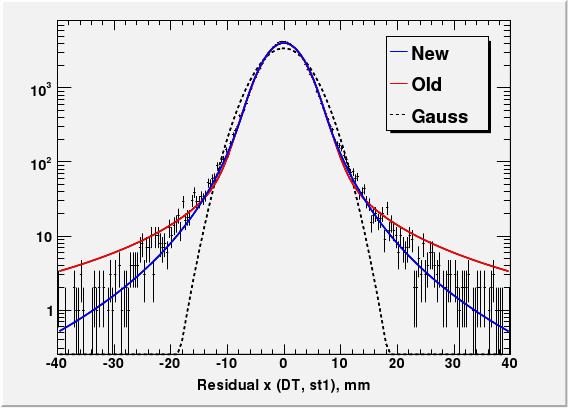
\includegraphics[width=\linewidth]{residuals_fit_functions.png}
\column{0.43\linewidth}
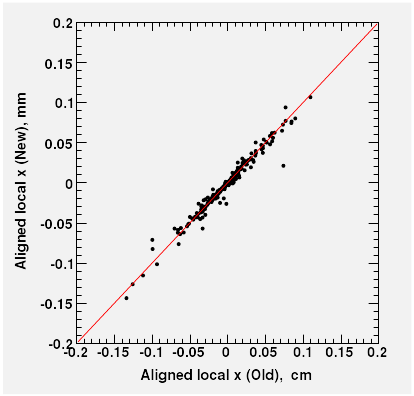
\includegraphics[width=\linewidth]{correlation_new_old.png}
\end{columns}
\end{frame}

\begin{frame}
\frametitle{Updated resolution vs.\ $\mathcal{L}$}

\begin{itemize}
\item Results of MC alignment challenge with $\mathcal{L}$ = 5--20~pb$^{-1}$: \\ vertical
  axis is RMS of aligned positions relative to true positions
\item Left: all chambers, dominated by stations with the broadest
  distribution (station~4); curves are $1/\sqrt{\mathcal{L}}$
\item Right: resolution of station~1 only (most important for track fit)
\end{itemize}

\begin{columns}
\column{0.5\linewidth}
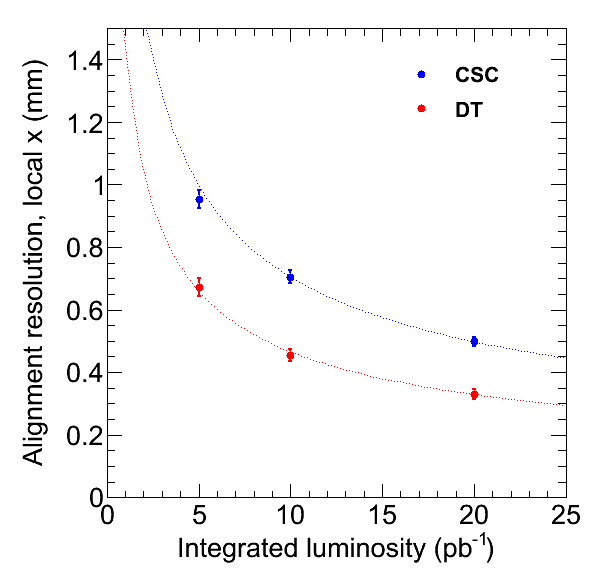
\includegraphics[width=\linewidth]{general_alignment_resolution.png}
\column{0.5\linewidth}
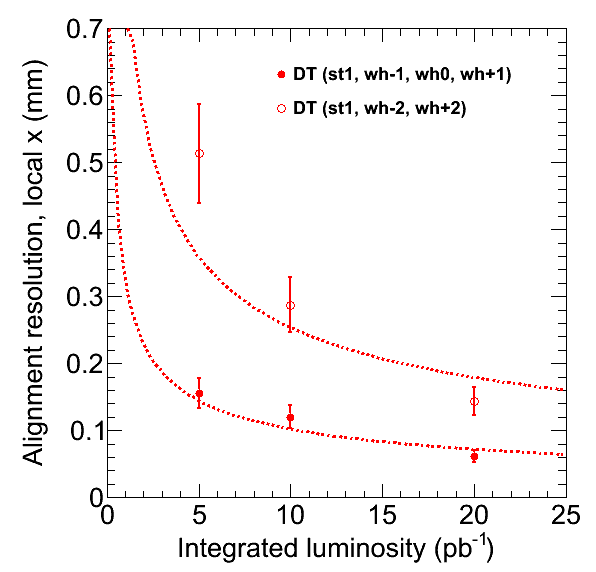
\includegraphics[width=\linewidth]{station1_resolution.png}
\end{columns}
\end{frame}

\begin{frame}
\frametitle{Dependence on momentum cut}

\begin{itemize}
\item Results on previous page require $p_T > 15$~GeV (imposed in ppMuX)

\item Loosening momentum cut adds more tracks for alignment but
  broadens residuals distribution (vs.\ $|p|$, not $p_T$); can be
  optimized

\item ppMuXLoose sample allows us to test resolution down to $p_T >
  2.5$~GeV, but $\mathcal{L} \approx 0.13$~pb$^{-1}$ in this sample

\item Advantage of more tracks outweighs broader distributions down to
  threshold, but it would be better to do this study with $\mathcal{L}
  \sim 5$~pb$^{-1}$
\end{itemize}

\begin{columns}
\column{0.5\linewidth}
\mbox{ } \hfill \textcolor{red}{DT station 1} \hfill \mbox{ }

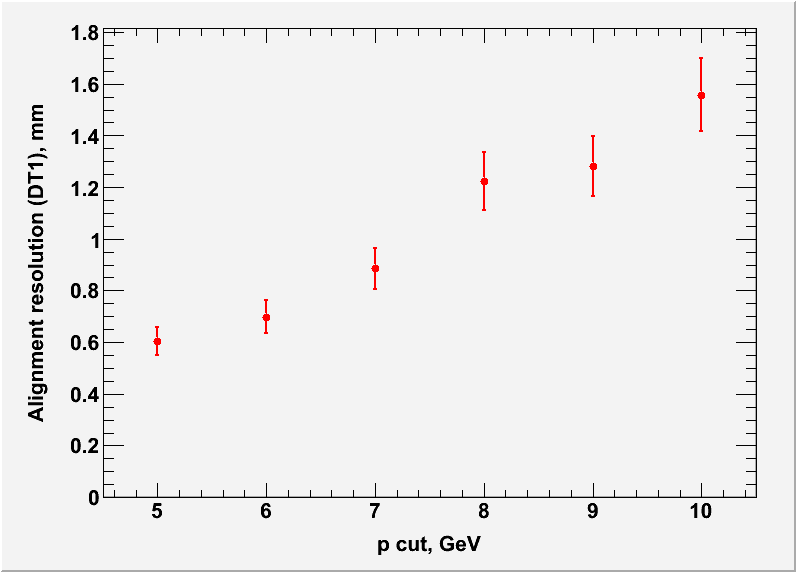
\includegraphics[width=\linewidth]{momentum_cut_study_dt.png}
\column{0.5\linewidth}
\mbox{ } \hfill \textcolor{blue}{CSC ME1/1} \hfill \mbox{ }

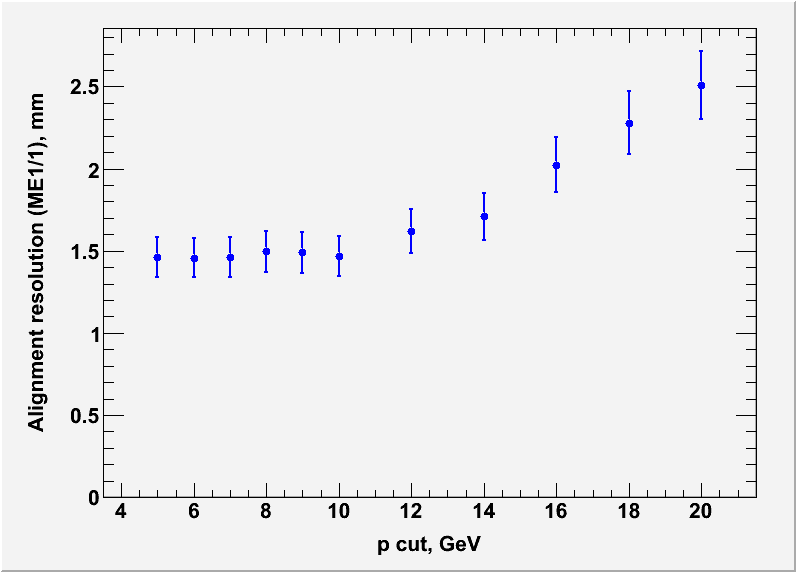
\includegraphics[width=\linewidth]{momentum_cut_study_csc.png}
\end{columns}

\hfill \textcolor{blue}{\scriptsize (in ME1/1, $p_T > 2.5$~GeV corresponds to $|p| > 10$~GeV)}
\end{frame}

\begin{frame}
\frametitle{Bias in input tracks (1/2)}

\begin{columns}
\column{0.35\linewidth}
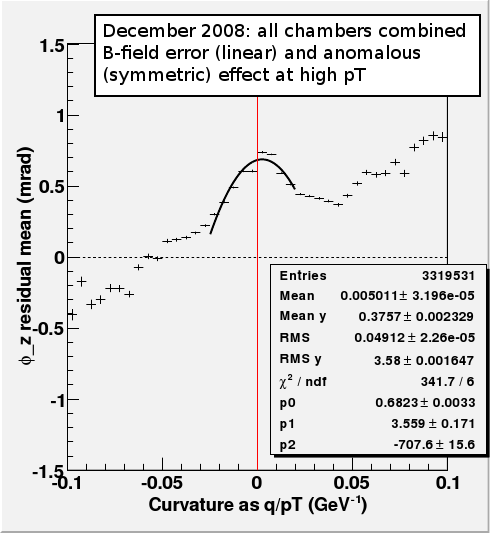
\includegraphics[width=\linewidth]{old_Deltax_vs_qoverpT.png}

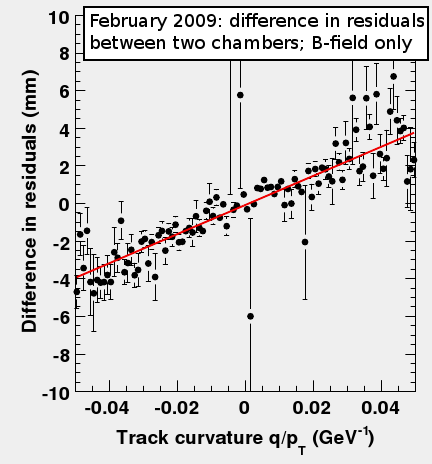
\includegraphics[width=\linewidth]{old_Deltax1-Deltax2_vs_qoverpT.png}

\column{0.65\linewidth}
\begin{itemize}
\item Muon residuals depend on input track momentum (shown as curvature, $q/p_T$)
\begin{itemize}
\item dependence is even present when plotted for a single DT layer (no influence from muon alignment)
\item linear dependence is $\vec{B}$-field error, which disappeared
  with the new $\vec{B}$-field maps (last spring)
\item anomalous (symmetric) effect at high-$p_T$ only present when
  propagating from the tracker, not between stations
\end{itemize}
\end{itemize}

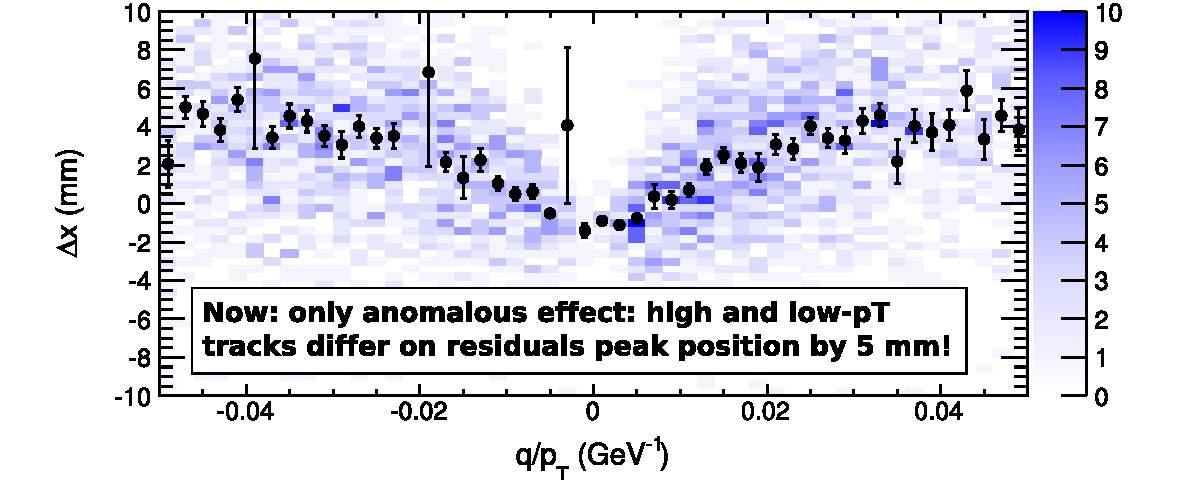
\includegraphics[width=\linewidth]{residuals_real.pdf}
\end{columns}
\end{frame}

\begin{frame}
\frametitle{Bias in input tracks (2/2)}

\begin{columns}
\column{0.65\linewidth}
\begin{itemize}
\item Markus Stoye generated a realistic example of a tracker weak mode
\begin{itemize}
\item coherent displacement of all tracker modules that does not
  affect the tracker-track $\chi^2$ distribution
\end{itemize}

\item This kind of distortion affects muon residuals with the same
  momentum behavior, even cancelling it at some $\phi$

\item Unfortunately, it does not cancel the effect for all $\phi$
  values; a slightly different mode would be \mbox{needed--- under investigation by the tracker alignment group\hspace{-5 cm}}
\end{itemize}

\column{0.35\linewidth}
\hfill \textcolor{darkblue}{M.~Stoye}

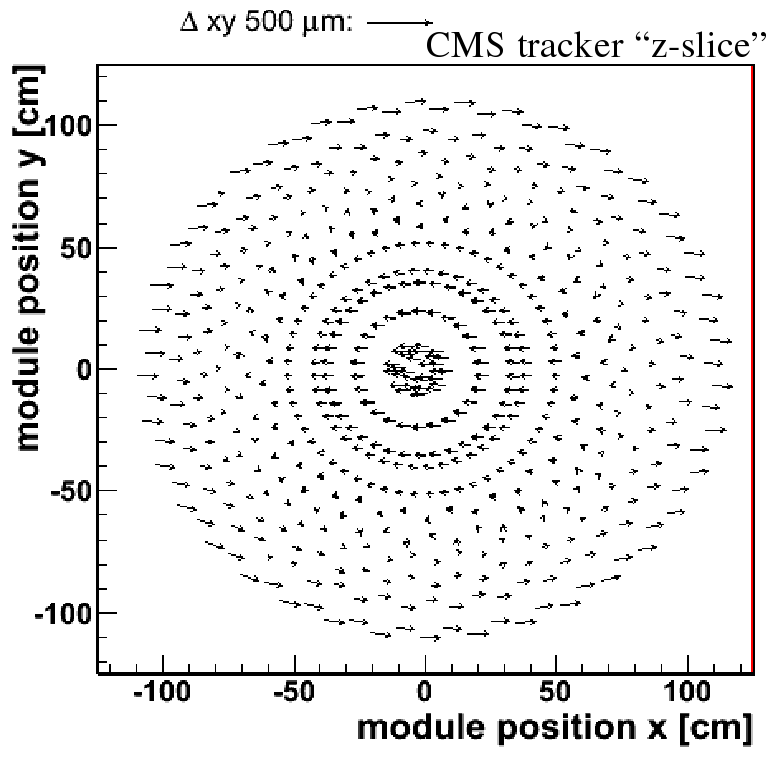
\includegraphics[width=\linewidth]{stoye_deformation.png}
\end{columns}

\vspace{0.25 cm}
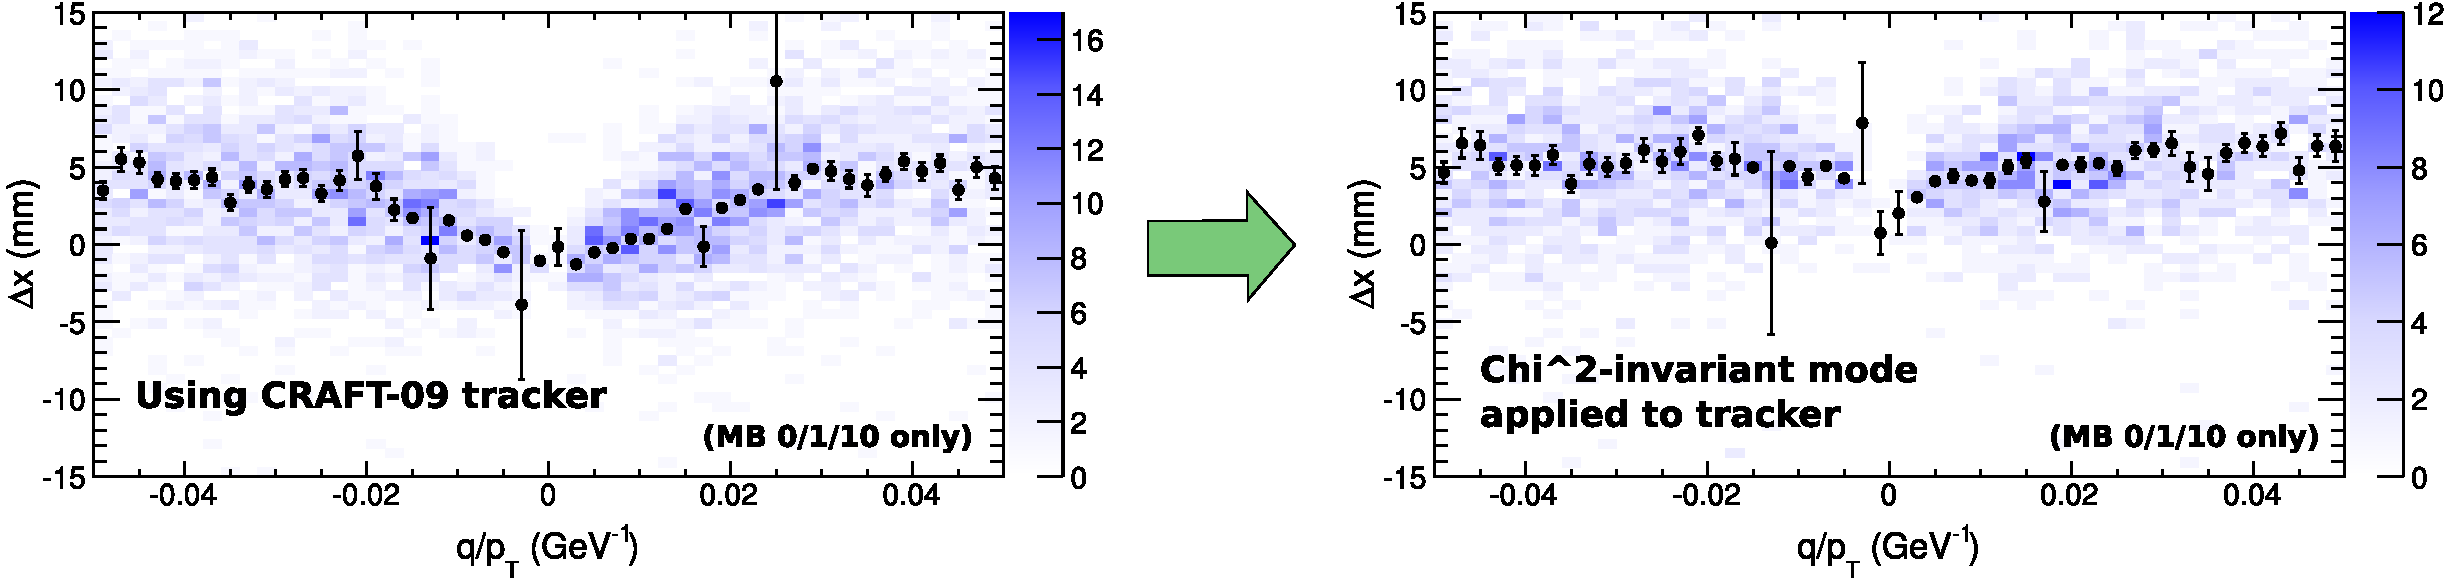
\includegraphics[width=\linewidth]{trackerMP3_weakmode.pdf}
\end{frame}

\begin{frame}
\frametitle{Relevance for muon alignment}

\begin{columns}
\column{0.5\linewidth}
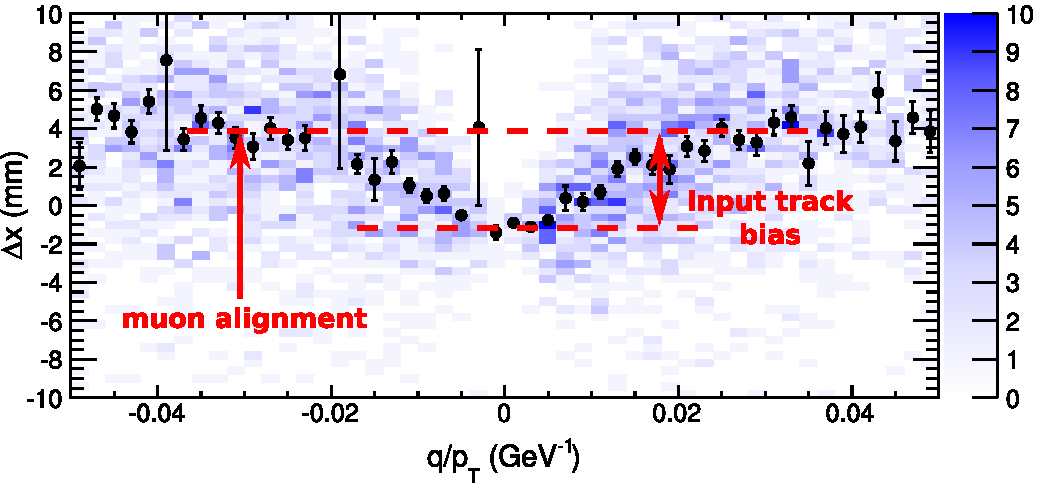
\includegraphics[width=1.1\linewidth]{residuals_breakup.pdf}

\column{0.5\linewidth}
\begin{itemize}
\item Input track bias can only be inferred from shape vs.\ momentum,
  not a constant offset in residuals, so we can only quantify {\it
    difference} between high-$p_T$ bias and low-$p_T$ bias
\end{itemize}
\end{columns}

{\hspace{0 cm}\begin{minipage}{1.2\linewidth}\scriptsize
$\displaystyle \mbox{bias}(p_T, \phi, \theta) - \mbox{bias}(0, \phi, \theta) = (5\times 10^{-4}\mbox{ GeV}^{-1}) \sin(\phi - 0.7) \exp\left(-\frac{(100\mbox{ GeV})^2}{{2 \, p_T}^2}\right)$
\end{minipage}\mbox{\hspace{-3 cm}}}

\begin{itemize}
\item External information from cosmic spectrum endpoint indicates
  that only about 10\% of the bias is in the high-momentum tracks

\mbox{ } \hfill {\scriptsize $\displaystyle \mbox{bias}(p_T \to \infty) \approx 5\times 10^{-5}$~GeV$^{-1}$} \hfill \mbox{ }

\item Hence, high-momentum tracks ($p_T > 100$~GeV) yield the most correct muon alignment
\begin{itemize}
\item we can align using high-momentum cosmic rays now
\item {\it but for alignments with collisions muons, the input-track bias must first be resolved!}
\end{itemize}
\end{itemize}
\end{frame}

\begin{frame}
\frametitle{New cosmic ray alignments}

\begin{itemize}
\item General strategy:
\begin{enumerate}
\item Reproduce CRAFT-09 alignment with the updated Reference-Target procedure
\item Align system with 2010 cosmic rays the same way
\end{enumerate}

\item CRAFT-09 constants reproduced within 30~$\mu$m (except for the 61 chambers that could not be aligned with the old Reference-Target)
\end{itemize}

\vfill
\mbox{ } \hfill 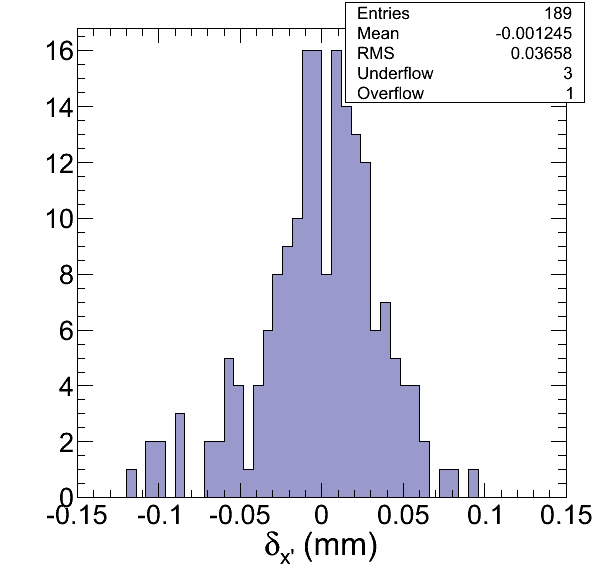
\includegraphics[width=0.5\linewidth]{craft09_redo3.png} \hfill \mbox{ }
\end{frame}

\begin{frame}
\frametitle{2010 cosmic ray data}

\begin{columns}
\column{0.35\linewidth}
\begin{itemize}
\item 2010 cosmics: about 80k $p_T > 100$~GeV tracks ($\frac{1}{3}$ of
  peak-mode CRAFT-09)

\item First alignment attempt resulted in unexpectedly few hits in
  sectors 2--6 (top of barrel)
\end{itemize}

\vspace{2 cm}

\column{0.7\linewidth}
From the alignment quality browser

\vspace{0.2 cm}
showing only $N_{\mbox{\scriptsize hits}} < 5$~warning (in yellow)

\vspace{0.2 cm}
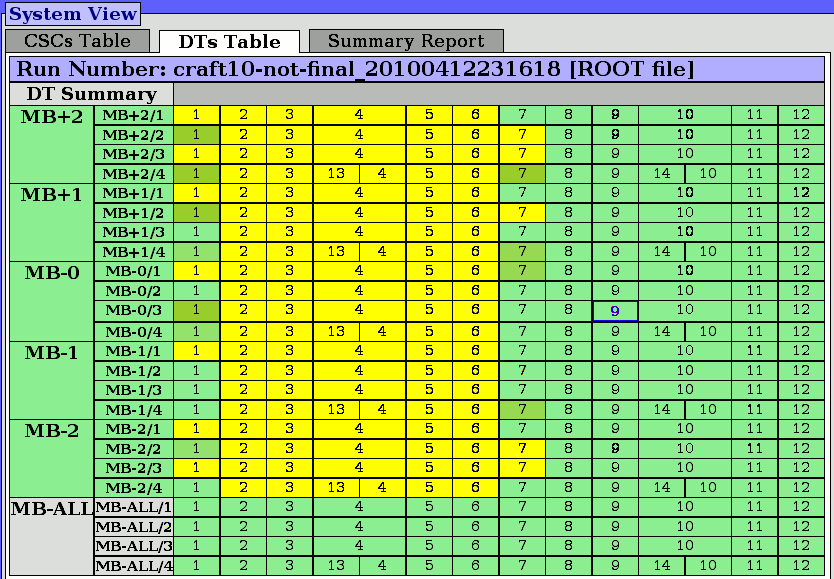
\includegraphics[width=\linewidth]{missing_top_hits.png}
\end{columns}
\end{frame}

\begin{frame}
\frametitle{Top tracks lost in refitting}

\begin{columns}
\column{0.5\linewidth}

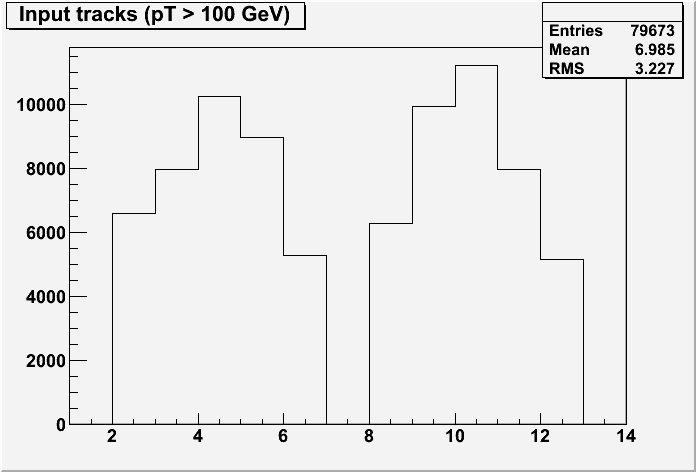
\includegraphics[width=\linewidth]{hits_i2_10.png}

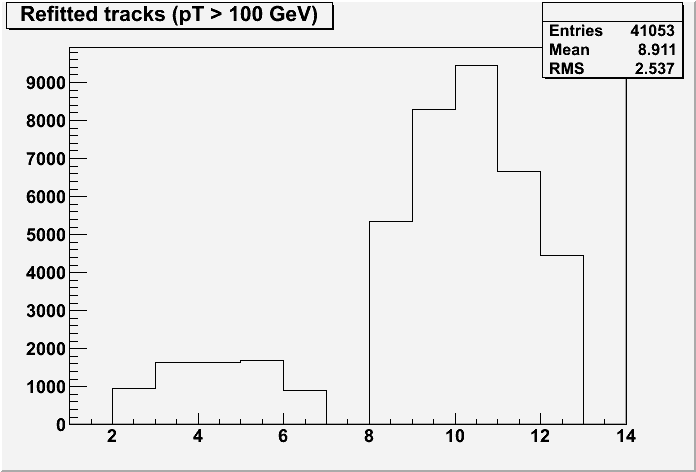
\includegraphics[width=\linewidth]{hits_r2_10.png}

\mbox{ } \hfill {\bf Sector number} \hfill \mbox{ }

\column{0.5\linewidth}
\begin{itemize}
\item Top hits were {\it not} lost in the trigger/data acquisition, but in the refitting stage (so this is recoverable)

\item Only 51\% of $p_T > 100$~GeV tracks successfully refit (compared to 99.7\% in CRAFT-09)

\item Preferentially drops tracks with top hits

\item We're attempting to use an old version of the refitter to isolate the problem (and communicating with the experts, of course :)
\end{itemize}

\end{columns}
\end{frame}

%% \section*{First section}
%% \begin{frame}
%% \begin{center}
%% \Huge \textcolor{blue}{First section}
%% \end{center}
%% \end{frame}

\begin{frame}
\frametitle{Conclusions}

\begin{itemize}
\item Reference-Target algorithm produces fit results with meaningful
  error bars for arbitrarily low statistics
\item MC results scale statistically; 5~pb$^{-1}$ ($p_T > 15$~GeV) yields
\begin{itemize}
\item $\sim$150~$\mu$m in station~1 wheels $-$1, 0, $+$1
\item $\sim$500~$\mu$m in station~1 wheels $\pm$2
\item $\sim$700~$\mu$m throughout barrel
\item $\sim$1~mm throughout muon system
\end{itemize}
and 20~pb$^{-1}$ yields $\sim$400~$\mu$m throughout barrel,
$\sim$500~$\mu$m throughout muon system

\vspace{0.1 cm}
{\it if there were no biases in the input tracks.}

\item Input track bias must be resolved before we can perform a muon
  alignment with low-momentum ($p_T \ll 100$~GeV) tracks

\item Cosmic rays remain the only source of high-momentum tracks

\item CRAFT-09 alignment reproduced and used as a test to diagnose
  refitting problems in 2010 cosmic ray alignment
\end{itemize}

\label{numpages}
\end{frame}

\begin{frame}
\begin{center}
\LARGE \textcolor{darkblue}{BACKUP}
\end{center}
\end{frame}

\begin{frame}
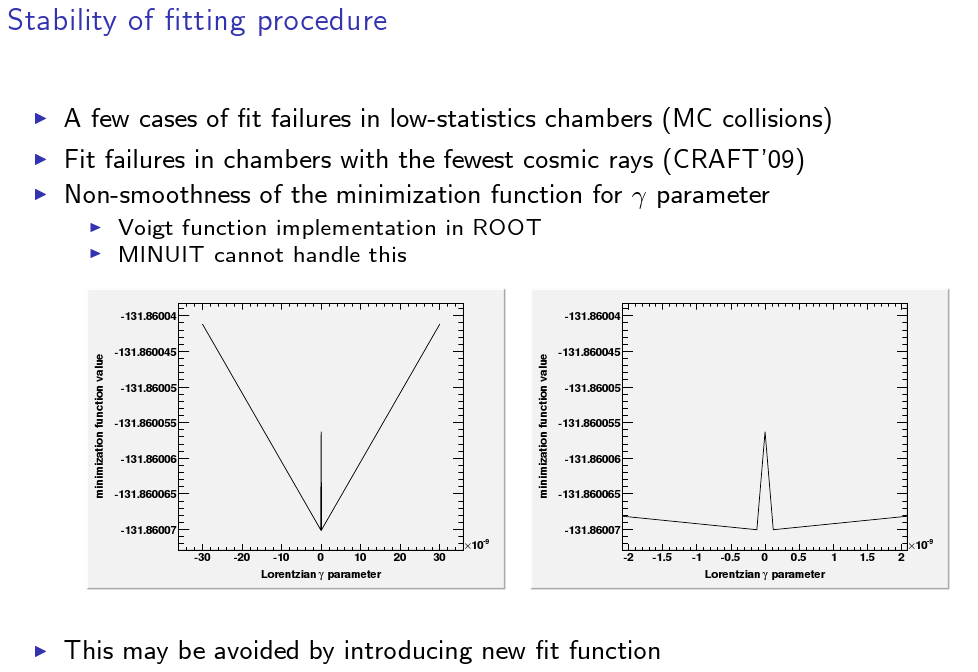
\includegraphics[width=\linewidth]{old_fit_function_gamma.png}
\end{frame}

\begin{frame}
\frametitle{Interpretation of this plot}

\begin{columns}
\column{0.5\linewidth}
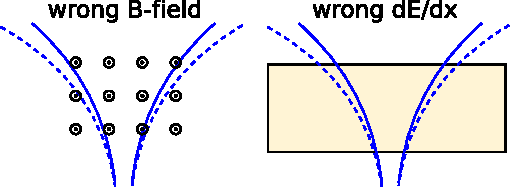
\includegraphics[width=\linewidth]{things_that_are_antisymmetric.pdf}

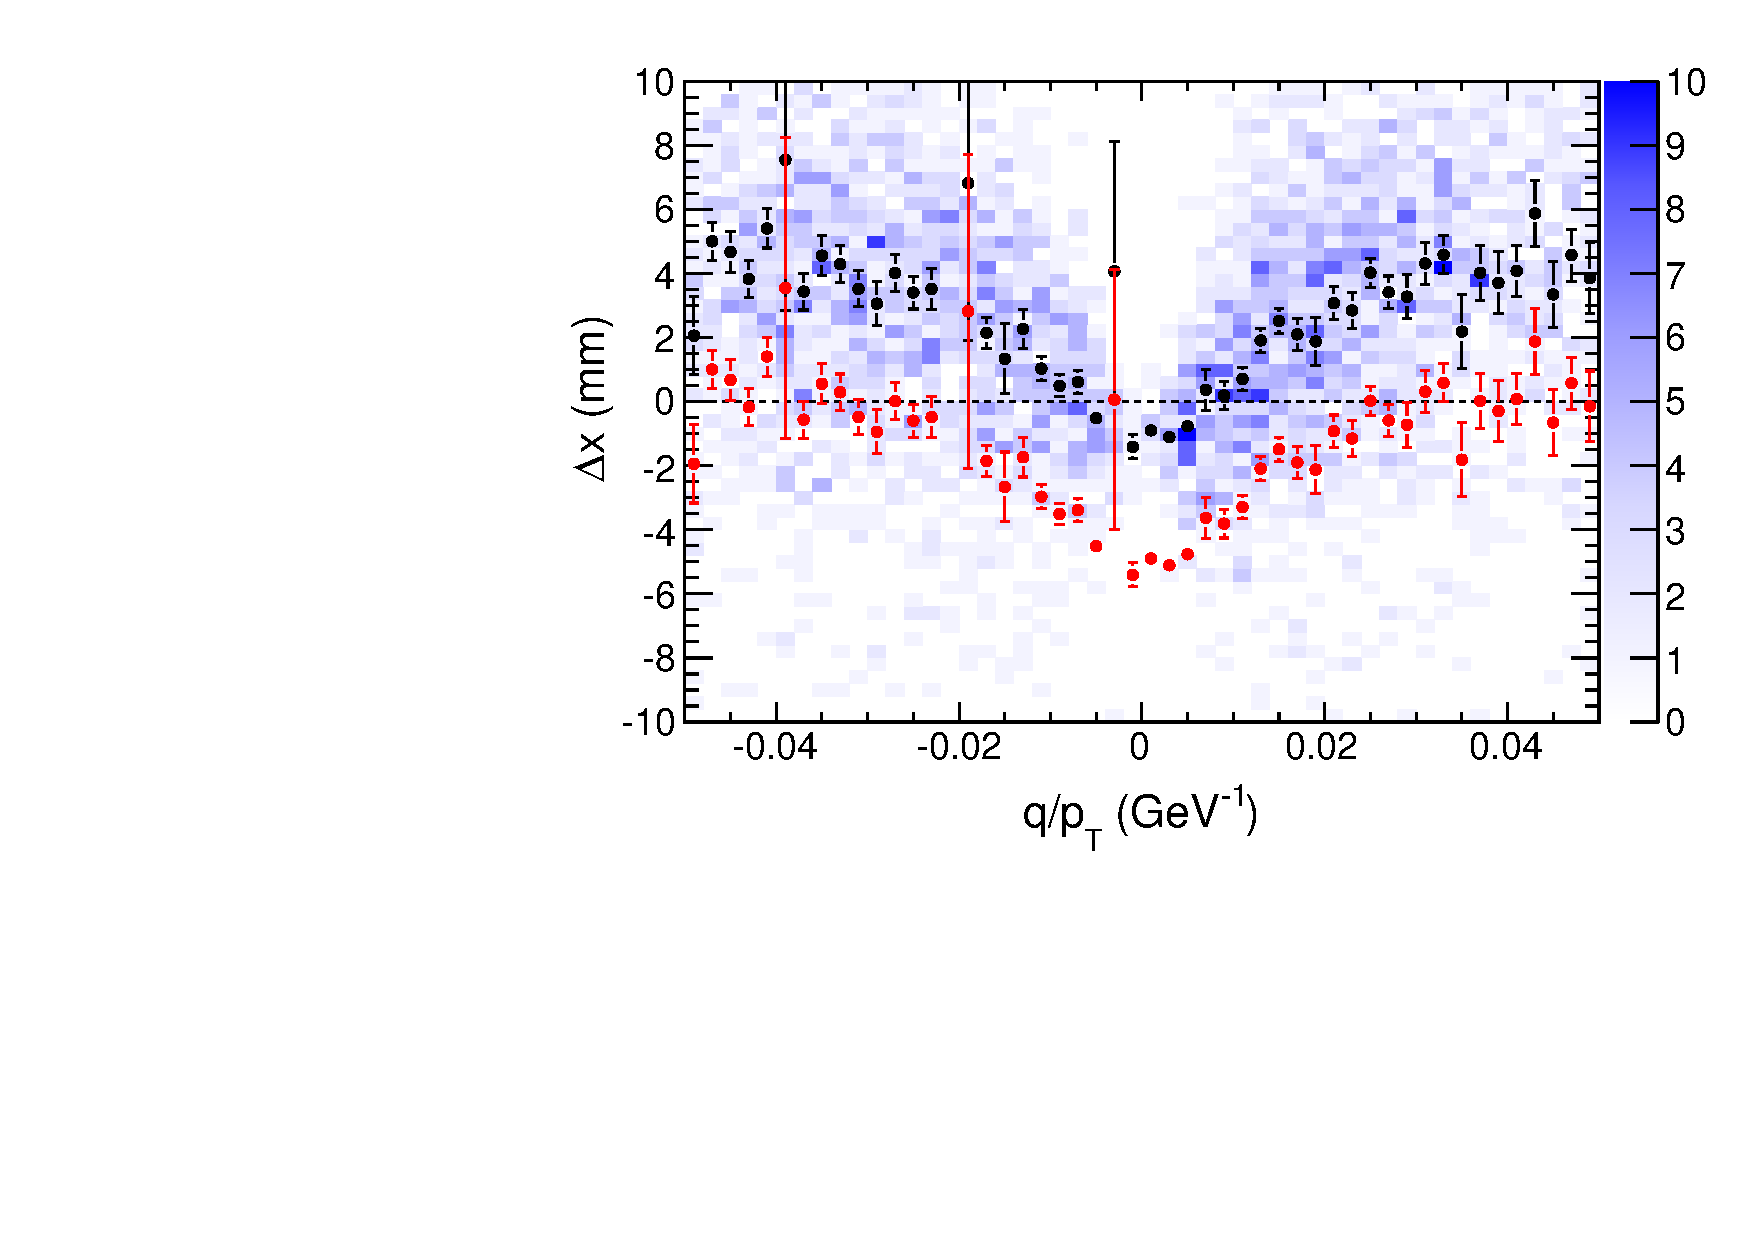
\includegraphics[width=\linewidth]{residuals_real_both.pdf}
\column{0.5\linewidth}
\begin{itemize}
\item Both magnetic field and material budget errors lead to antisymmetric effects on $\Delta x$
\begin{itemize}
\item high-momentum feature effect is therefore neither
\end{itemize}
\item When it is made with a single muon layer, layer misalignment (in
  $r\phi$) corresponds to vertical translation
\begin{itemize}
\item ignore vertical offsets
\end{itemize}
\end{itemize}
\end{columns}

\begin{itemize}
\item Transform $\displaystyle \Delta(q/p_T) = \frac{\epsilon}{x(q/p_T)
  - x(q/p_T + \epsilon)} \Delta x$, numerical \\ \vspace{0.2 cm} derivative calculated by
  running propagator twice (purely mathematical); $\Delta(q/p_T)$ vs $q/p_T$ quantifies tracker only
\end{itemize}
\end{frame}

\begin{frame}
\frametitle{{\large Parameterization and combined fit}}
\framesubtitle{using the $\Delta(q/p_T)$ plots and expanding the expression to include wheels}

$(A)\kappa + \big[(F + F_{\theta}\cot\theta) + $

\hfill $(S + S_{\theta}\cot\theta)\sin(\phi) + (C + C_{\theta}\cot\theta)\cos(\phi)\big]\exp(-\kappa^2 W^2 / 2)$

\begin{center}
$\chi^2/N_{dof} = 2194/1066 = 2.06$
\end{center}
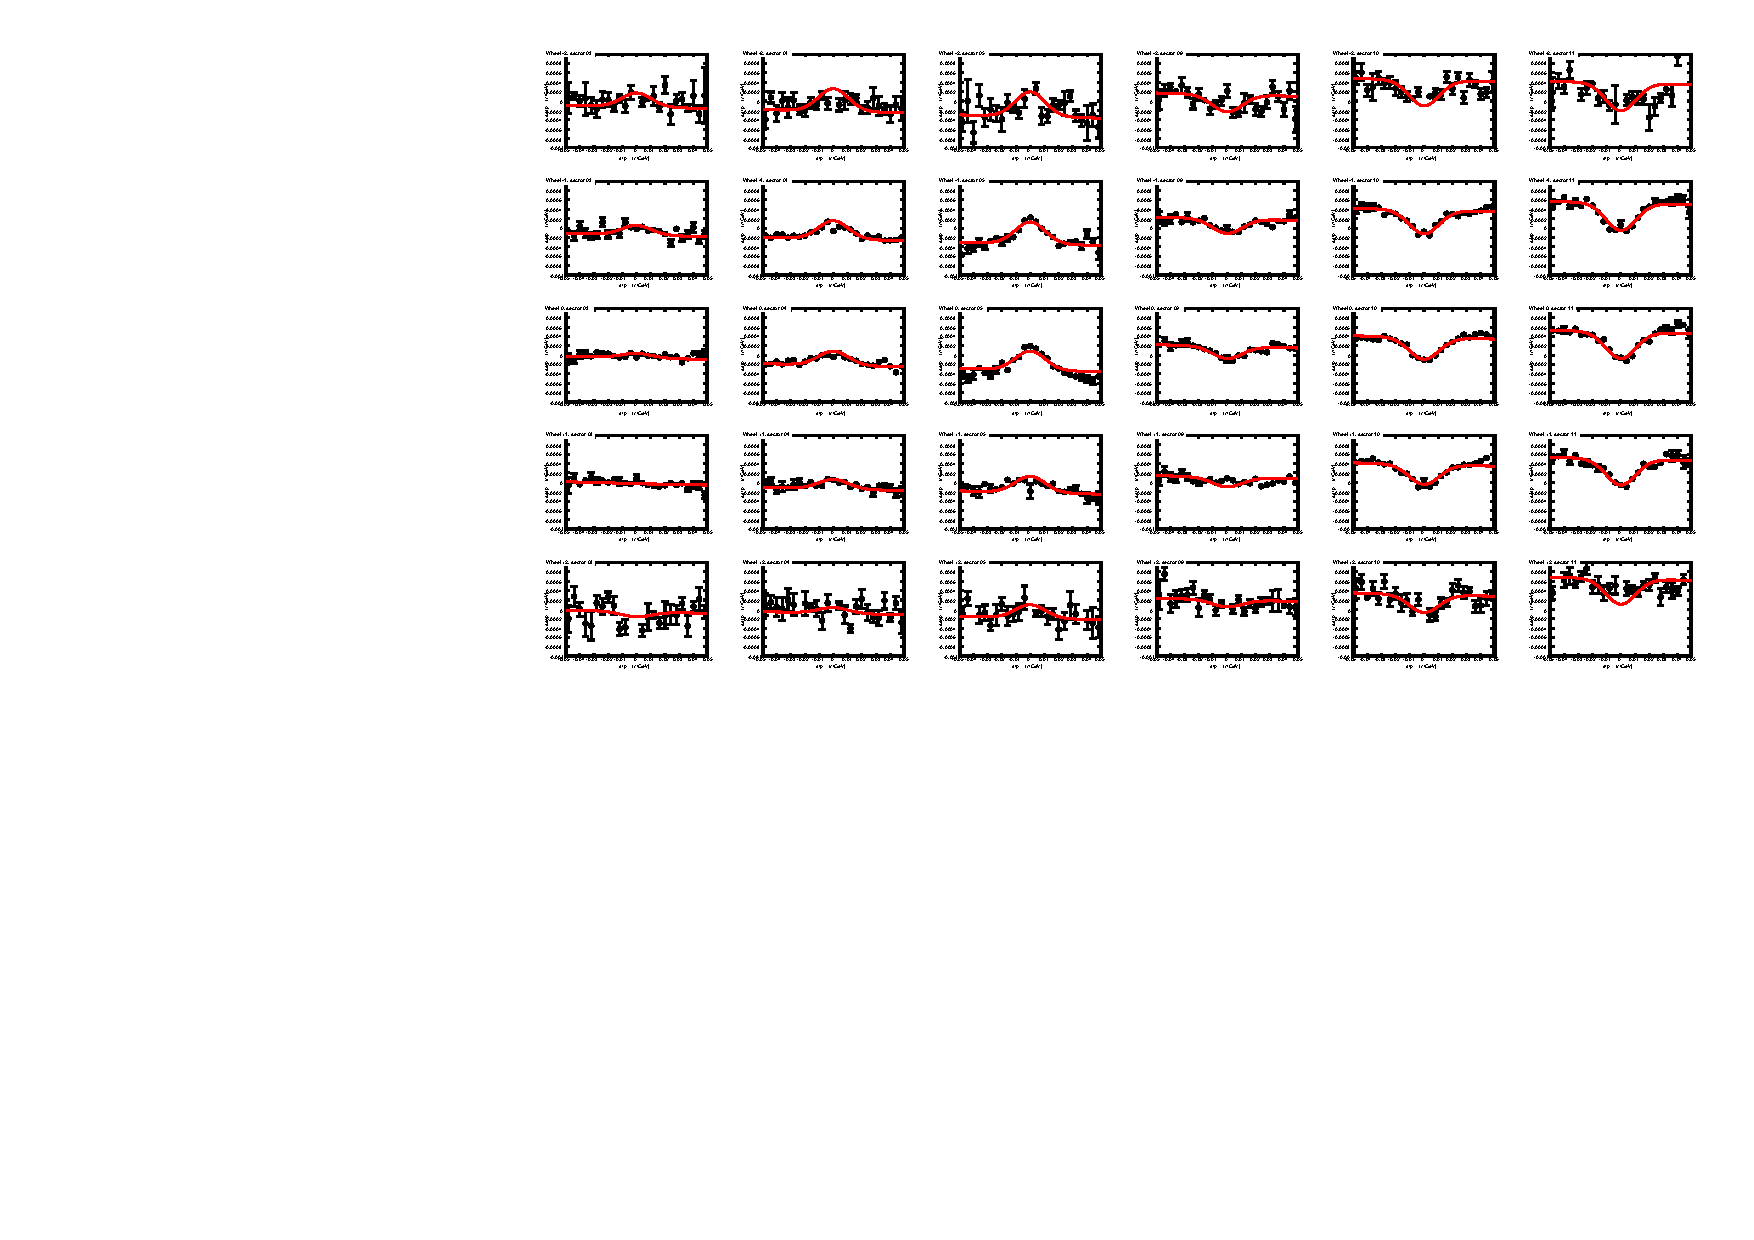
\includegraphics[width=0.9\linewidth]{allfits.pdf}
\end{frame}

\begin{frame}
\frametitle{{\large Millepede-generated mode} {\normalsize (M.~Stoye)}}

\begin{columns}
\column{0.6\linewidth}
\begin{columns}
\column{0.5\linewidth}
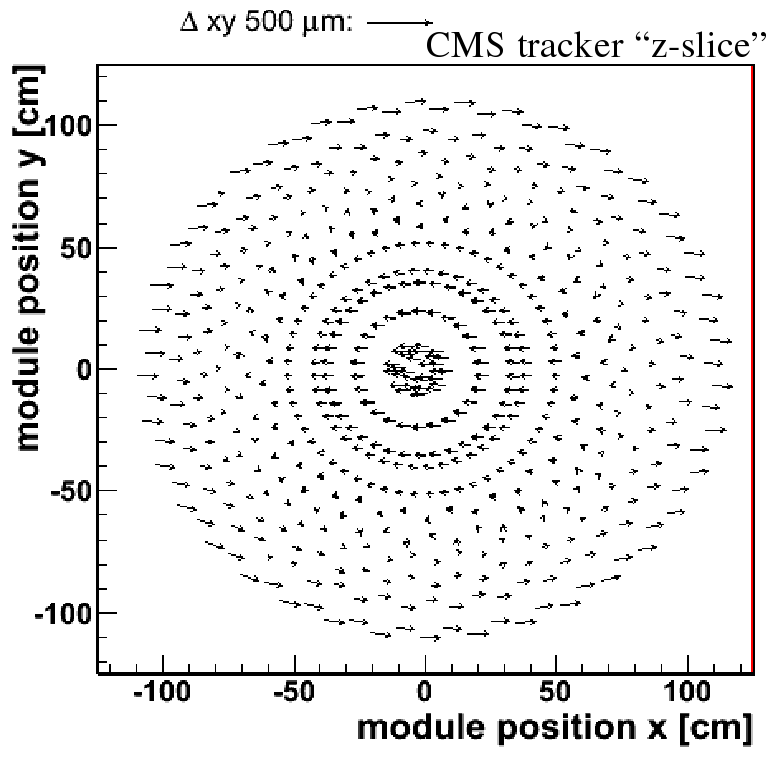
\includegraphics[width=\linewidth]{stoye_deformation.png}
\column{0.5\linewidth}
\only<1>{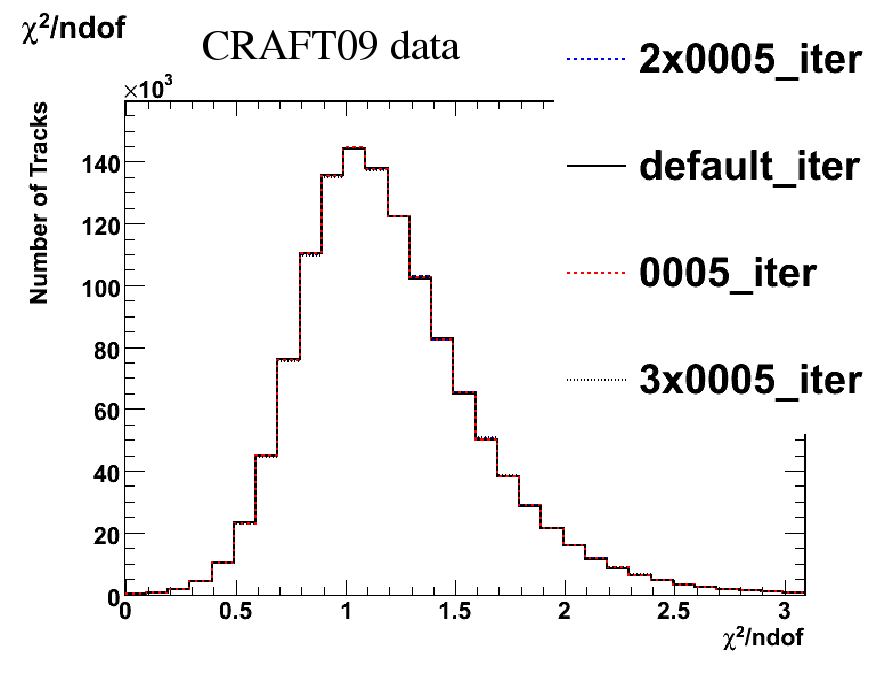
\includegraphics[width=\linewidth]{chi2_invariance.png}}
\only<2>{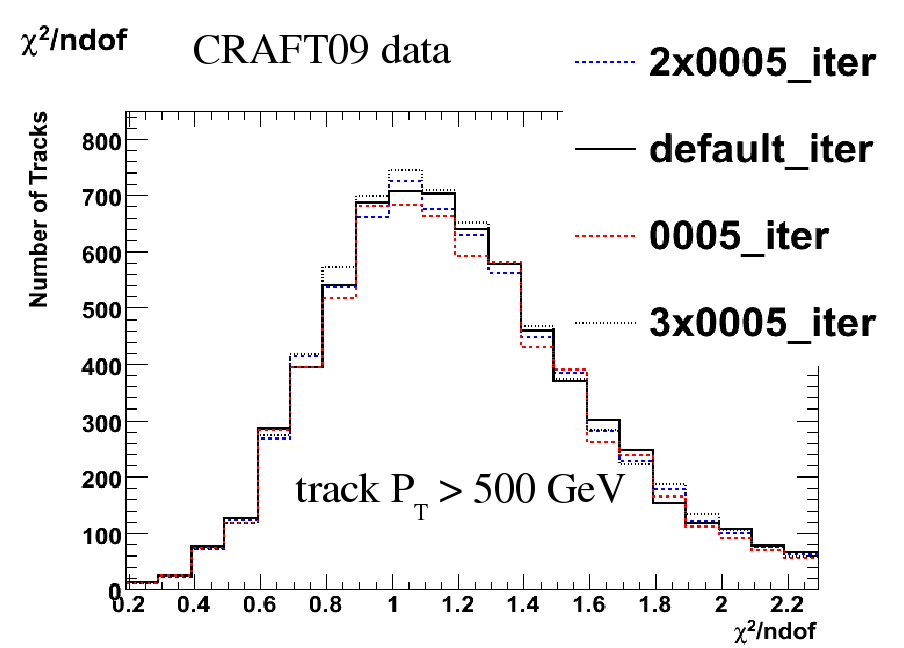
\includegraphics[width=\linewidth]{chi2_invariance_highpt.png}}
\end{columns}

\column{0.4\linewidth}
\begin{itemize}
\item Coherent distortion of tracker with no tracker $\chi^2$ sensitivity

\item We can see its effect with muon reisduals
\end{itemize}
\end{columns}

\vfill
\scriptsize

$(A)\kappa + \big[(F + F_{\theta}\cot\theta) + (S + S_{\theta}\cot\theta)\sin(\phi) + (C + C_{\theta}\cot\theta)\cos(\phi)\big]\exp(-\kappa^2 W^2 / 2)$

\vfill

\begin{tabular}{l r r r r}
 & $\chi^2/N_{dof}$ & $A$\hspace{0.35 cm} & $F$ (GeV$^{-1}$) & $F_{\theta}$ (GeV$^{-1}$) \\\hline
mode$\times$0 & 2194/1066 & $-0.000\,70$ & $-0.000\,082$ & $-0.000\,039$ \\
mode$\times$1 & 2171/1068 & $-0.000\,63$ & $0.000\,098$ & $-0.000\,063$  \\
mode$\times$3 & 1991/942 & $-0.000\,68$ & $0.000\,277$ & $-0.000\,070$ \\\hline
uncertainty & & $0.000\,09$ & $0.000\,005$ & $0.000\,009$ \\
\end{tabular}

\vfill
\hfill \begin{tabular}{l r r r r r}
& $S$ (GeV$^{-1}$) & $S_{\theta}$ (GeV$^{-1}$) & $C$ (GeV$^{-1}$) & $C_{\theta}$ (GeV$^{-1}$) & $W$ (GeV) \\\hline
mode$\times$0 & $0.000\,3533$ & $-0.000\,113$ & $-0.000\,345$ & $-0.000\,057$ & $95.0$ \\
mode$\times$1 & $0.000\,3892$ & $-0.000\,156$ & $-0.000\,335$ & $-0.000\,063$ & $93.1$ \\
mode$\times$3 & $0.000\,4310$ & $-0.000\,170$ & $-0.000\,386$ & $-0.000\,096$ & $84.1$ \\\hline
uncertainty & $0.000\,0064$ & $0.000\,011$ & $0.000\,010$ & $0.000\,016$ & 2.1 \\
\end{tabular}
\end{frame}

\begin{frame}
\frametitle{Graphical presentation}

\scriptsize

$(A)\kappa + \big[(F + F_{\theta}\cot\theta) + (S + S_{\theta}\cot\theta)\sin(\phi) + (C + C_{\theta}\cot\theta)\cos(\phi)\big]\exp(-\kappa^2 W^2 / 2)$

\vfill

\begin{tabular}{l r r r r}
 & $\chi^2/N_{dof}$ & $A$\hspace{0.35 cm} & $F$ (GeV$^{-1}$) & $F_{\theta}$ (GeV$^{-1}$) \\\hline
mode$\times$0 & 2194/1066 & $-0.000\,70$ & $-0.000\,082$ & $-0.000\,039$ \\
mode$\times$1 & 2171/1068 & $-0.000\,63$ & $0.000\,098$ & $-0.000\,063$  \\
mode$\times$3 & 1991/942 & $-0.000\,68$ & $0.000\,277$ & $-0.000\,070$ \\\hline
uncertainty & & $0.000\,09$ & $0.000\,005$ & $0.000\,009$ \\
\end{tabular}

\vfill
\hfill \begin{tabular}{l r r r r r}
& $S$ (GeV$^{-1}$) & $S_{\theta}$ (GeV$^{-1}$) & $C$ (GeV$^{-1}$) & $C_{\theta}$ (GeV$^{-1}$) & $W$ (GeV) \\\hline
mode$\times$0 & $0.000\,3533$ & $-0.000\,113$ & $-0.000\,345$ & $-0.000\,057$ & $95.0$ \\
mode$\times$1 & $0.000\,3892$ & $-0.000\,156$ & $-0.000\,335$ & $-0.000\,063$ & $93.1$ \\
mode$\times$3 & $0.000\,4310$ & $-0.000\,170$ & $-0.000\,386$ & $-0.000\,096$ & $84.1$ \\\hline
uncertainty & $0.000\,0064$ & $0.000\,011$ & $0.000\,010$ & $0.000\,016$ & 2.1 \\
\end{tabular}

\begin{center}
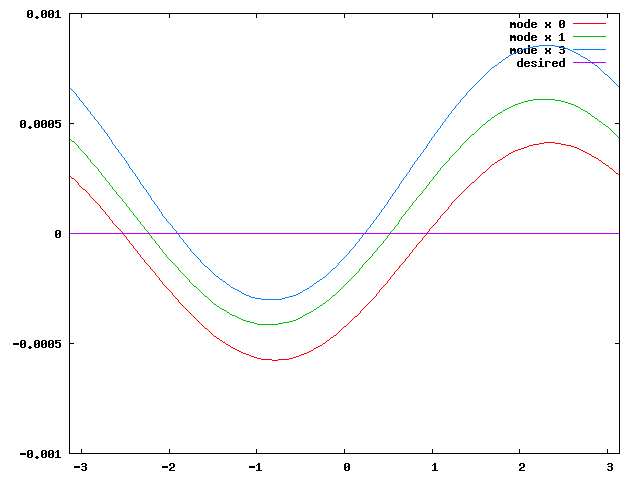
\includegraphics[width=0.4\linewidth]{modes.png}
\end{center}
\end{frame}

\begin{frame}
\frametitle{Absolute curvature bias}
\begin{itemize}
\item If we could know the absolute curvature bias of either high or
  low momentum tracks, we could use the muon residuals to predict
  to the other

\hfill 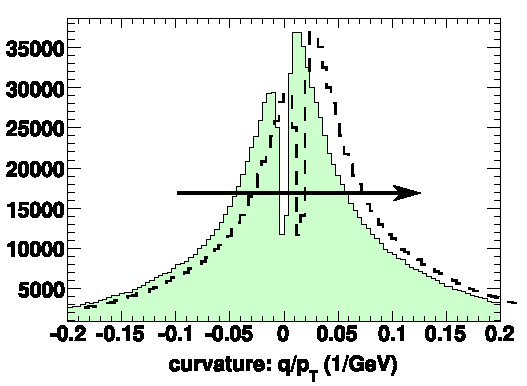
\includegraphics[width=0.4\linewidth]{biases.pdf}

\vspace{-3 cm}
\item Cosmics endpoint: assuming $\sim$flat \\ efficiency for
  high-momentum muons, \\ cosmic ray spectrum in $q/p_T$ must \\ point at
  zero (they trail off to infinite \\ momentum)
\begin{itemize}
\item identifies high-momentum \\ constant offset in $\Delta(q/p_T)$ vs $q/p_T$ (next slide)
\end{itemize}

\item Known resonance masses: identify linear slope in low-momentum $\Delta(q/p_T)$ vs $q/p_T$

\item Curvature of tracks in zero magnetic field: identify constant offset in low-momentum $\Delta(q/p_T)$ vs $q/p_T$

\item $K_S \to \pi^+\pi^-$ decay direction constraint: identify constant offset in low-momentum $\Delta(q/p_T)$ vs $q/p_T$ (following slides)
\end{itemize}
\end{frame}

\begin{frame}
\frametitle{Cosmics endpoint {\normalsize (I.~Furi\'c)}}

\begin{columns}
\column{0.65\linewidth}
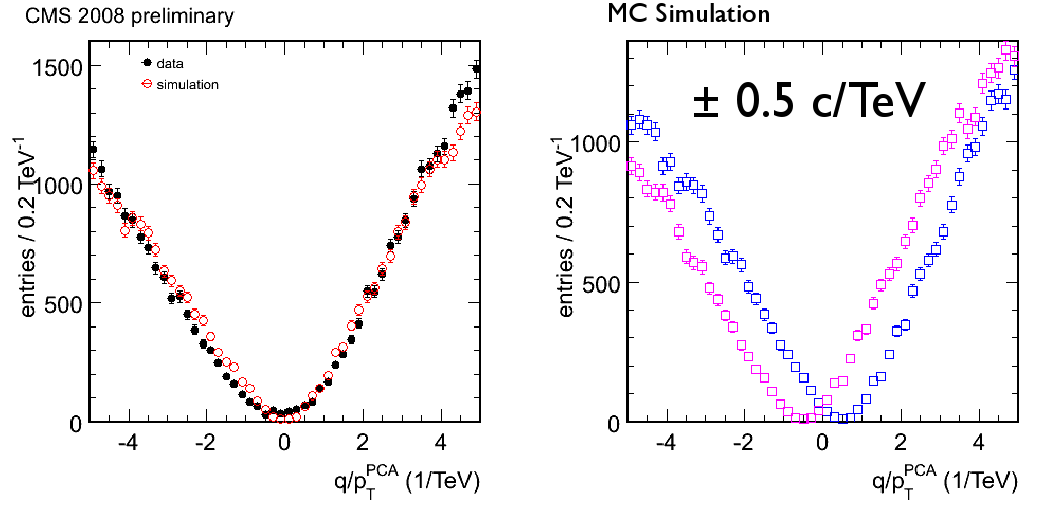
\includegraphics[width=\linewidth]{ivan_cosmic_endpoint.png}

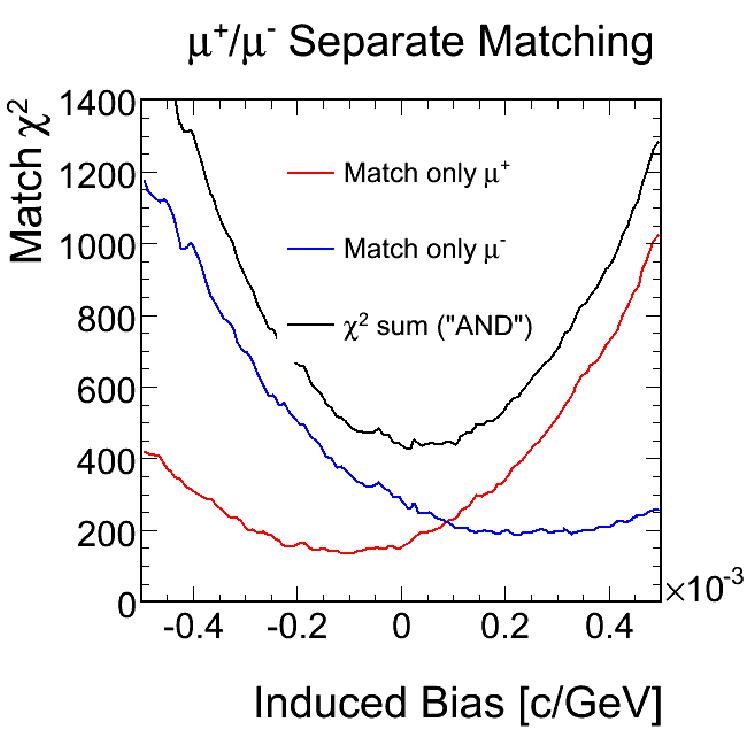
\includegraphics[width=0.7\linewidth]{ivan_chi2.png}
\column{0.5\linewidth}
\begin{itemize}
\item Distribution of cosmic rays trail off at high $p_T$, so positive
  and negative distributions must both point to $q/p_T = 0$ (infinite momentum)

\item Doesn't assume charge ratio, only shape of spectrum (well-known ``energy$^{-2.7}$'')

\item Data are most consistent with $\sim 5\times 10^{-5}$~GeV$^{-1}$, ten times
  smaller than $\mbox{bias}(\mbox{high}) - \mbox{bias}(\mbox{low})$ = \\ \hfill $5\times 10^{-4} \sin\phi$~GeV$^{-1}$

\item Implies that the muon-residuals effect is mostly in $\Delta \kappa(\mbox{low})$?  Can we check that?

\end{itemize}
\end{columns}
\end{frame}

\begin{frame}
\frametitle{{\large $K_S \to \pi^+\pi^-$ direction constraint}}

\begin{itemize}
\item Momentum sum of the $\pi^+\pi^-$ system must be collinear with
  the displacement of the secondary vertex

\item As a constraint on momenta, this is orthogonal to resonance mass
\end{itemize}

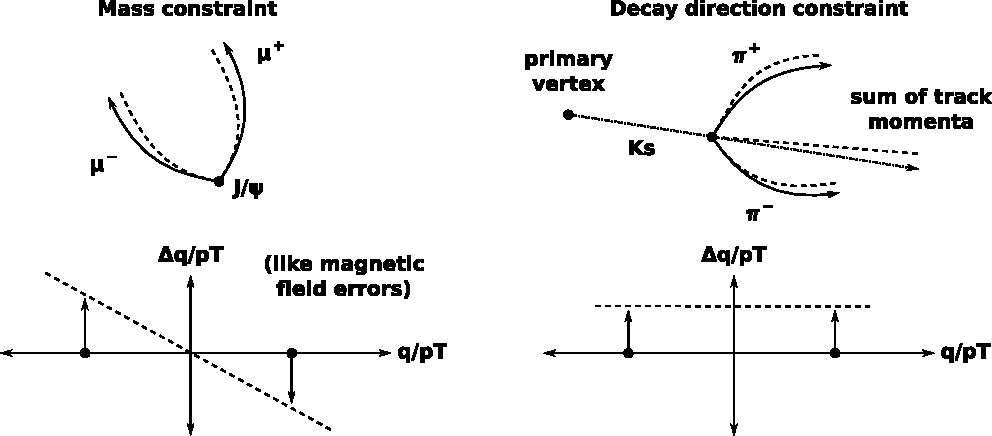
\includegraphics[width=\linewidth]{diagram.pdf}

\begin{itemize}
\item These two are the first terms in a general $\Delta \kappa(\kappa, \phi, \theta)$ expansion in $\kappa$

\end{itemize}
\end{frame}

\begin{frame}
\frametitle{Implementing the $K_S$ constraint}
\framesubtitle{to get a sense of how tight it is from Nov-Dec 2009 data}

\hfill 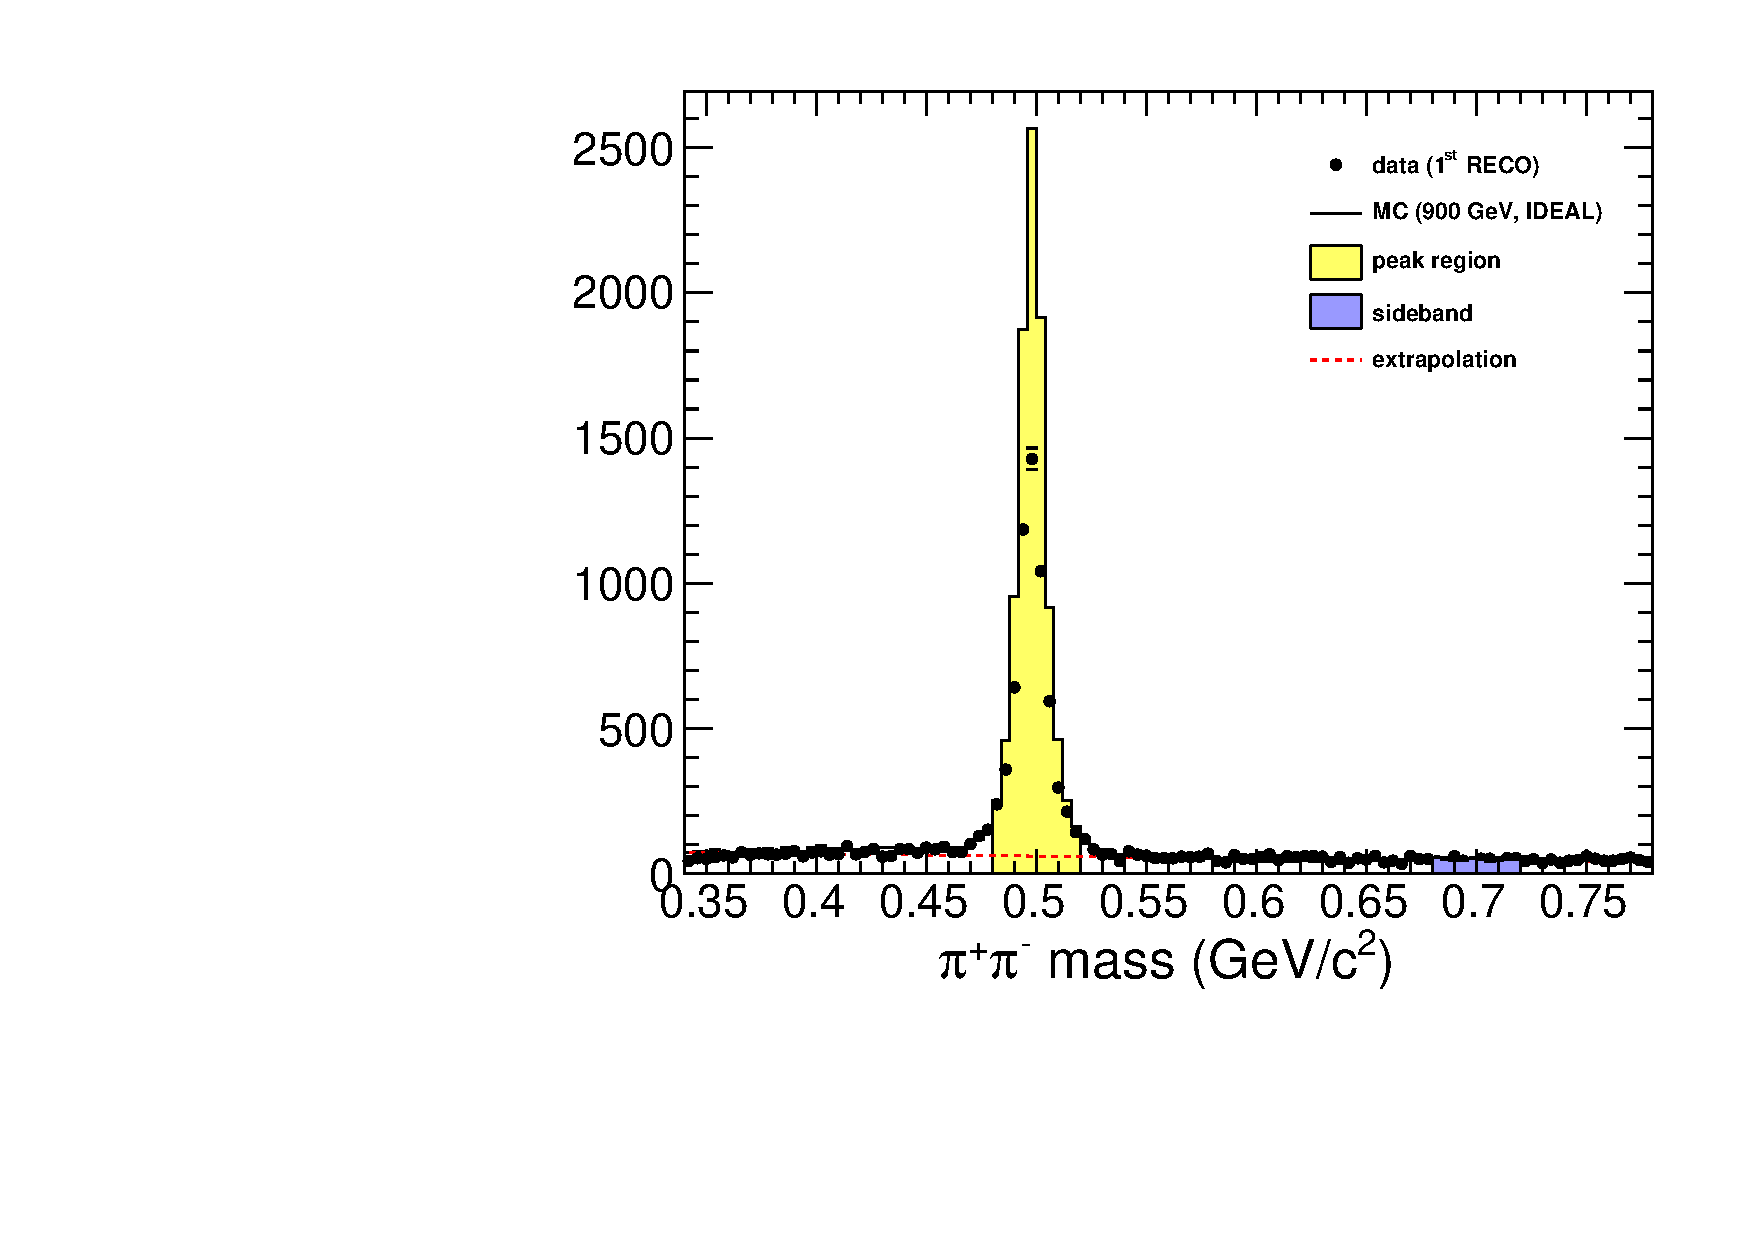
\includegraphics[width=0.5\linewidth]{kaonTracking2_masspeak.pdf}

\vspace{-4.6 cm}
\begin{itemize}
\item Select events using
\begin{itemize}
\item $\pi^+\pi^-$ mass with \\ sideband subtraction
\item vertex inside the first \\ pixel layer
\end{itemize}
\item Pointing to choose the primary \\ vertex in $z$ projection
\end{itemize}

\hspace{1 cm} 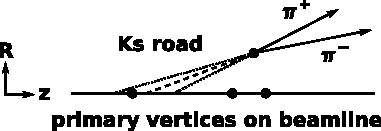
\includegraphics[width=0.3\linewidth]{diagram2.pdf}

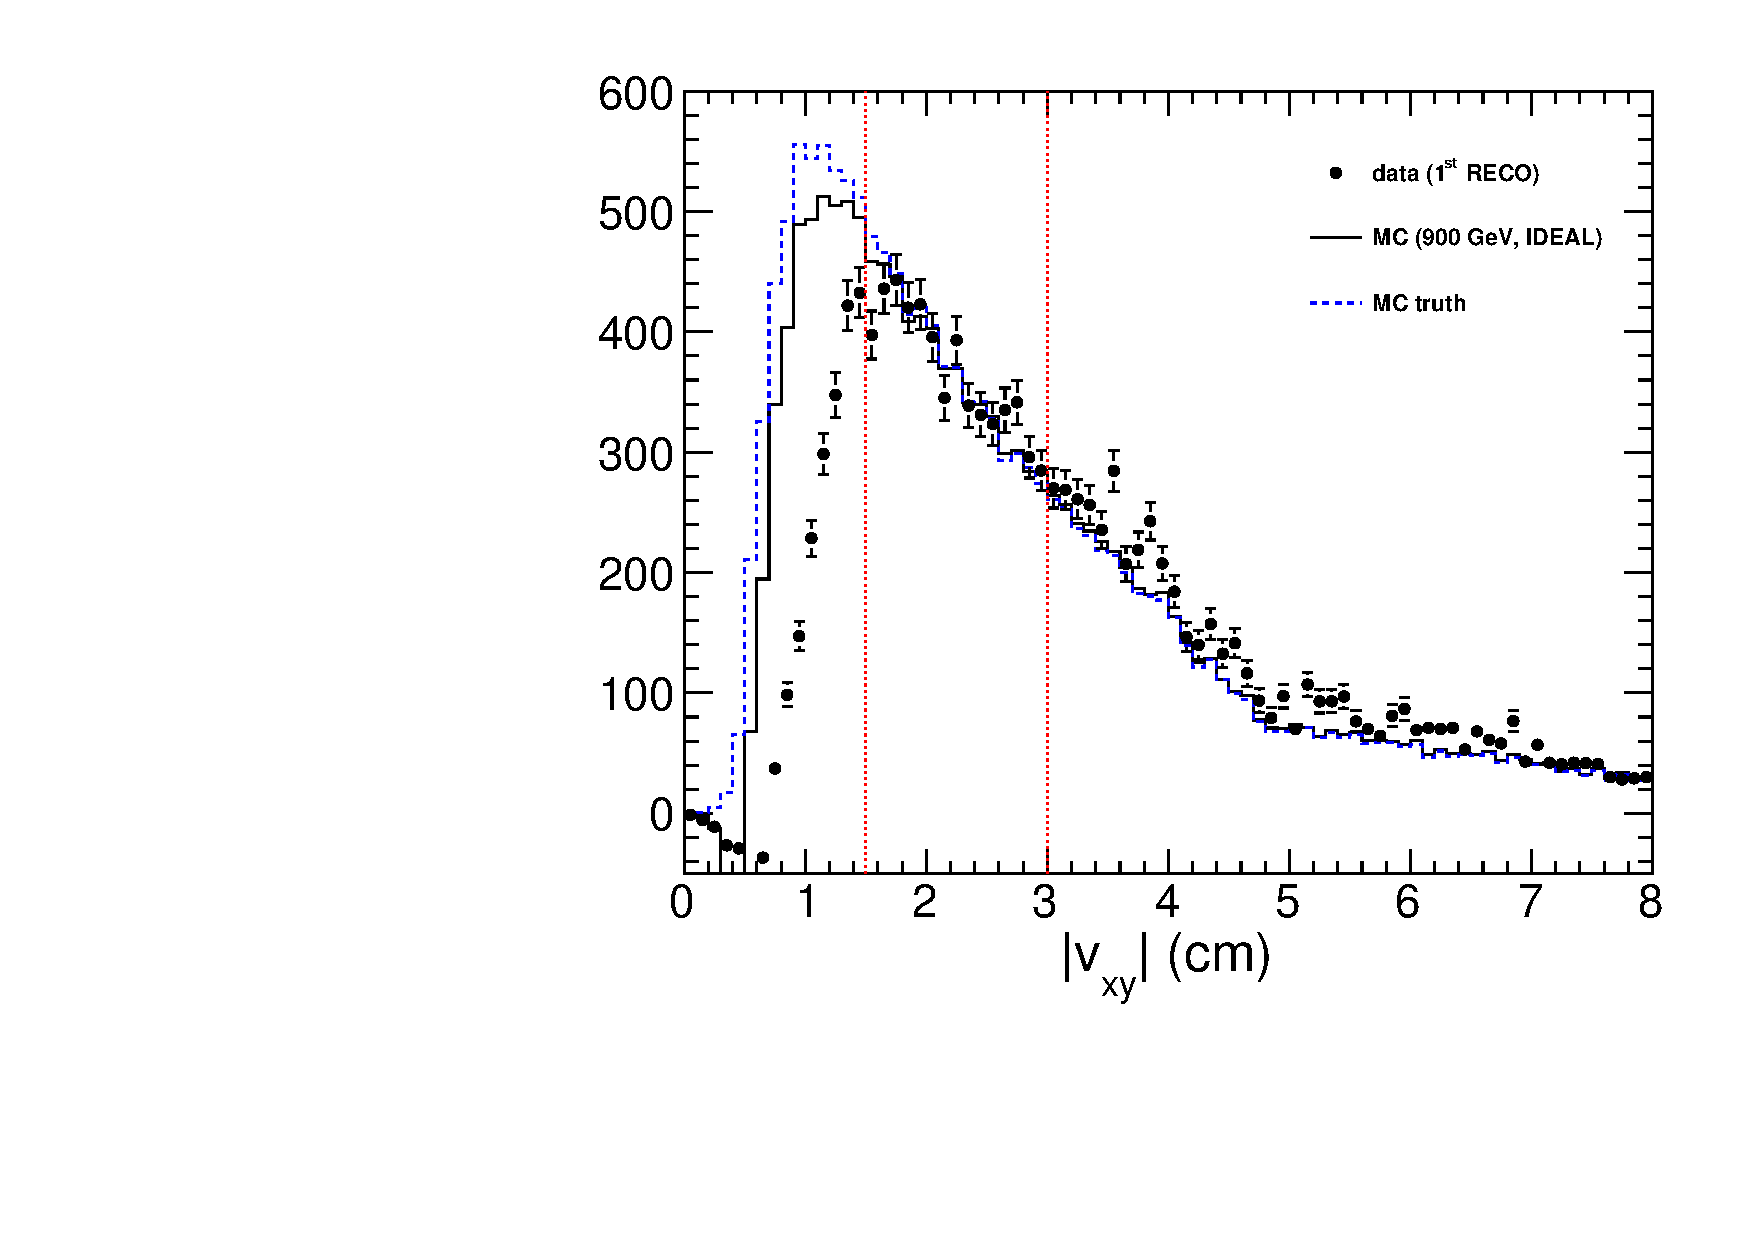
\includegraphics[height=3.5 cm]{kaonTracking2_vxy.pdf}
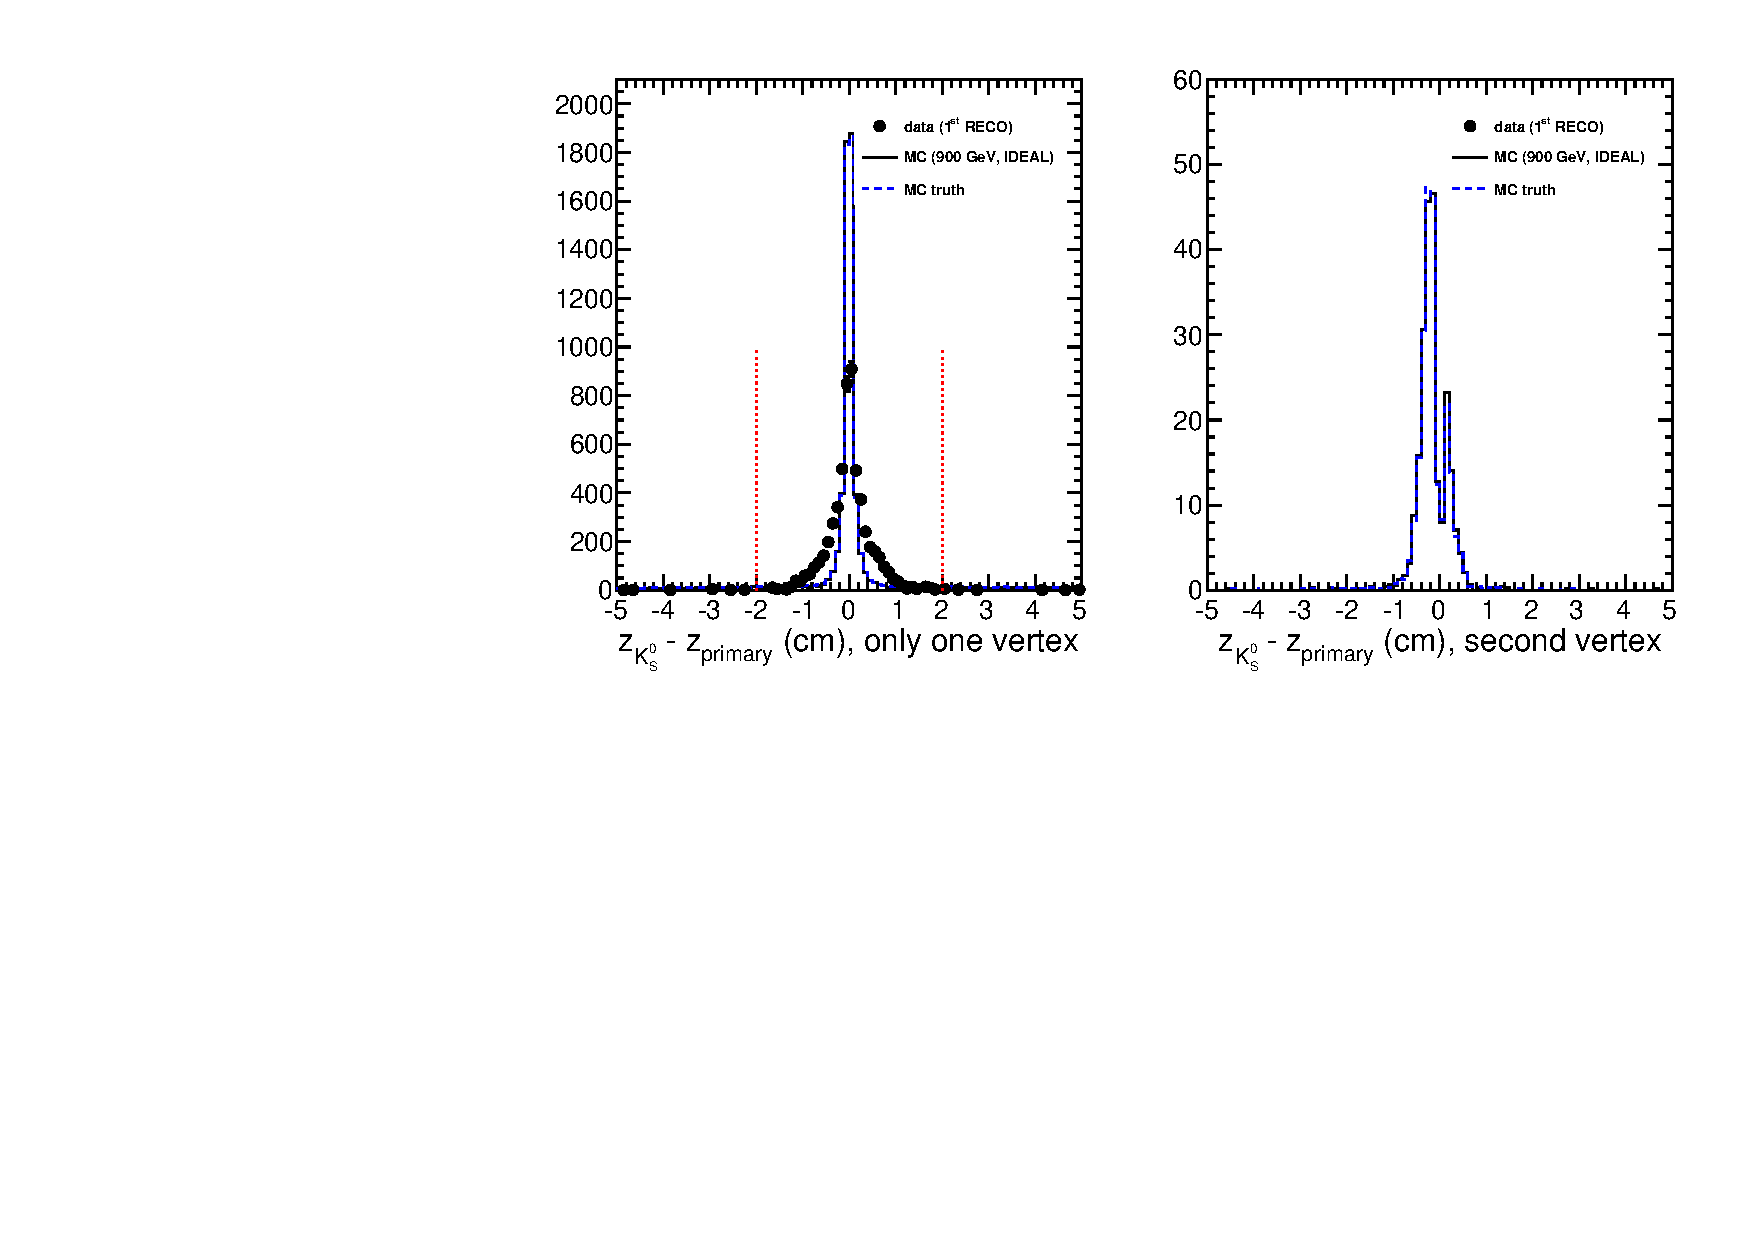
\includegraphics[height=3.5 cm]{kaonTracking2_zcut.pdf}
\end{frame}

\begin{frame}
\frametitle{Observable: $\Delta \phi$}

\begin{itemize}
\item Angle between primary-to-secondary displacement vector and $\pi^+\pi^-$ momentum sum in the transverse plane: $\Delta \phi$

\item Not used up by any selection requirements
\end{itemize}

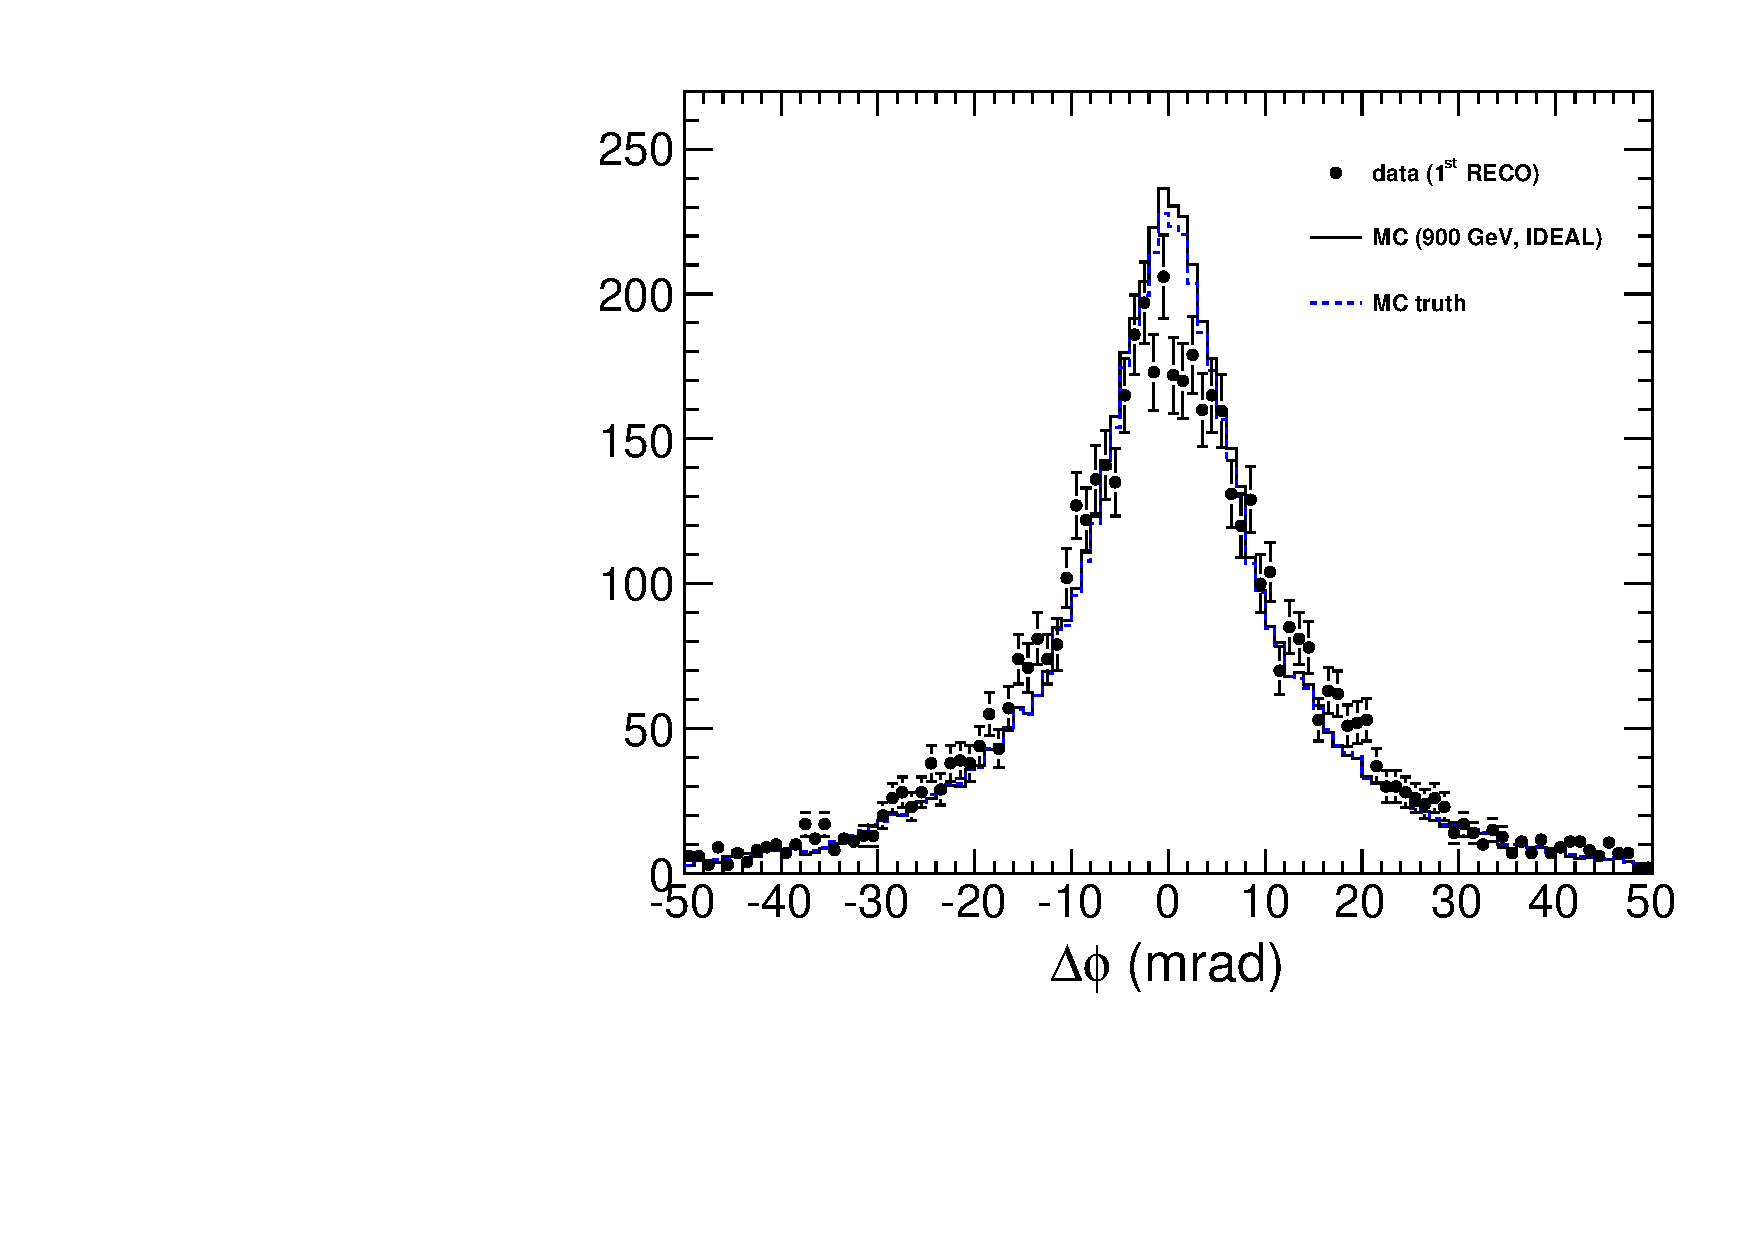
\includegraphics[width=0.5\linewidth]{kaonTracking2_deltaphi.pdf}
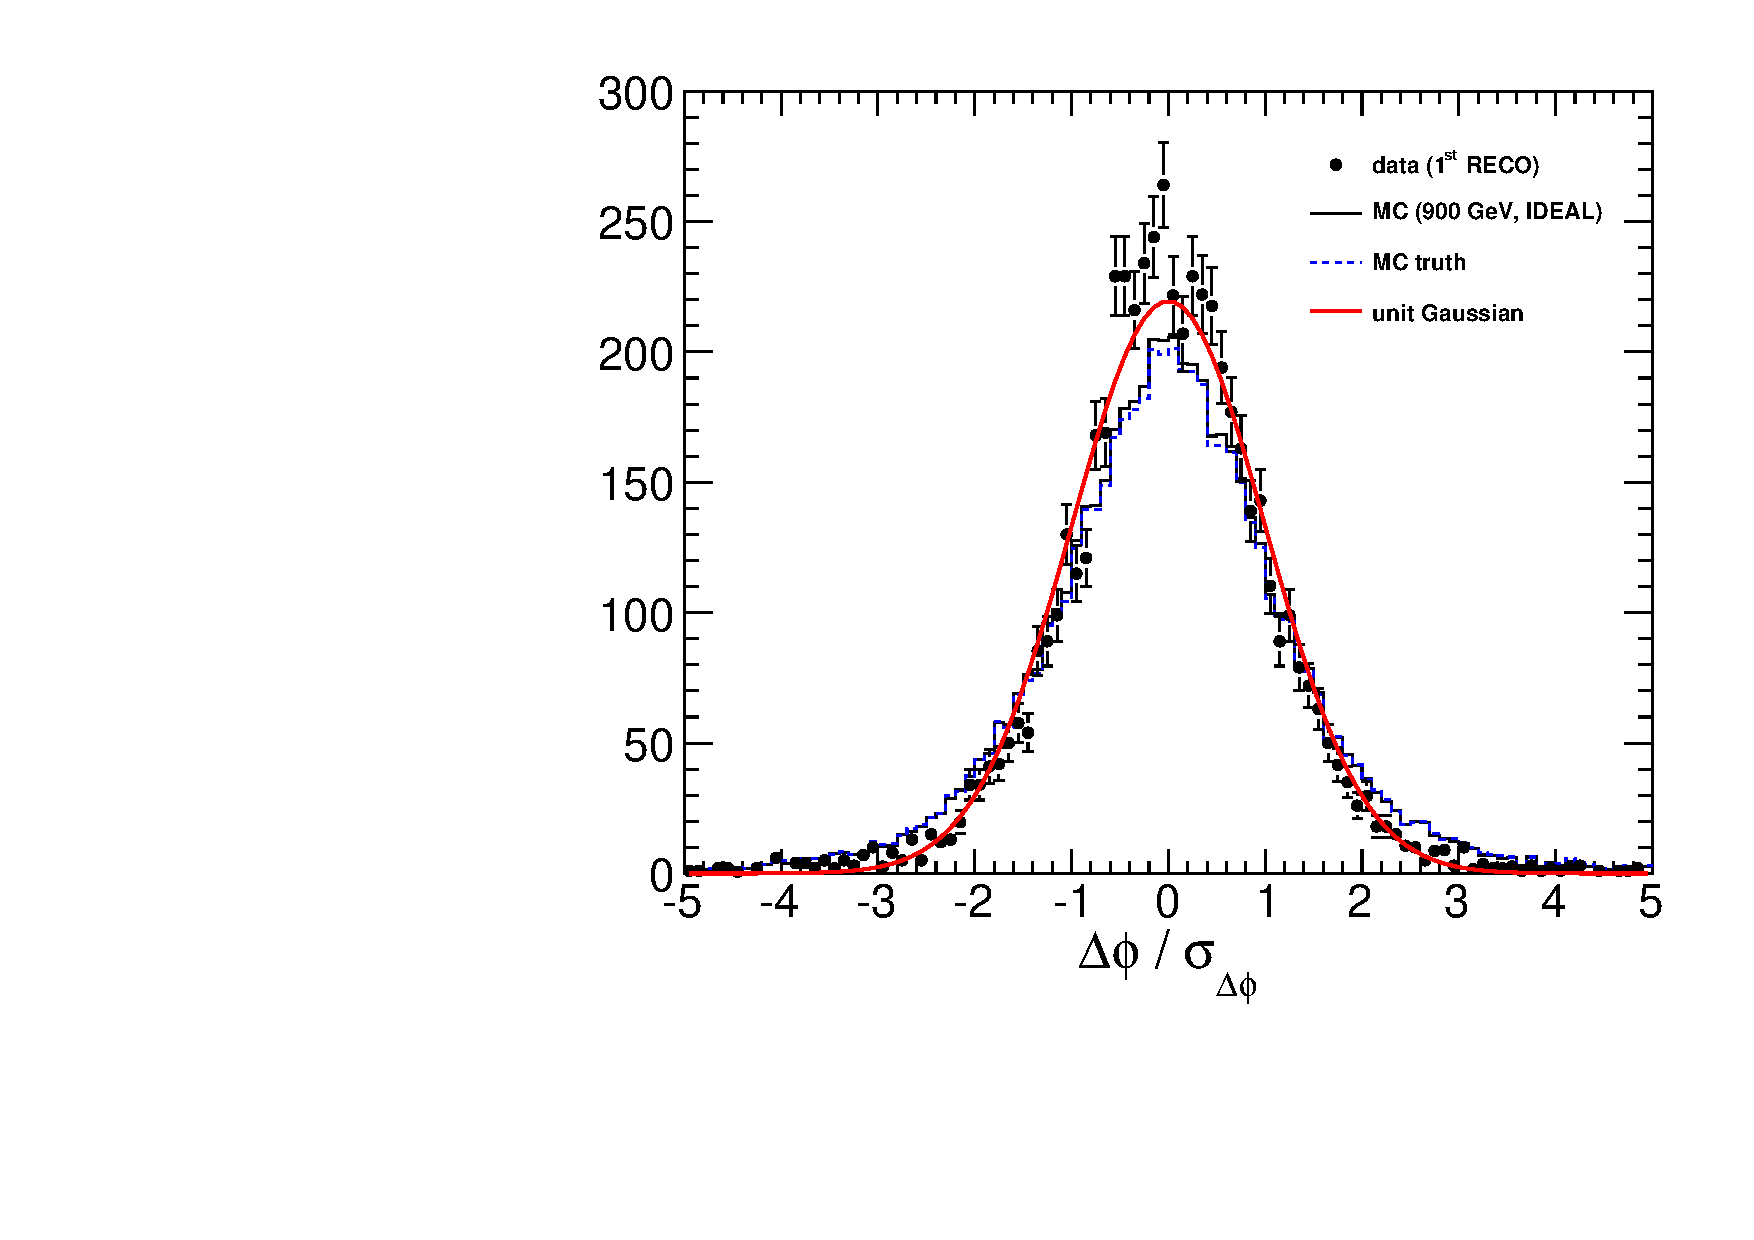
\includegraphics[width=0.5\linewidth]{kaonTracking2_normalized.pdf}

\begin{itemize}
\item No observed bias, with some uncertainty
\end{itemize}
\end{frame}

\begin{frame}
\frametitle{Convert to absolute $\Delta(q/p_T)$}

\begin{itemize}
\item Compute $\frac{\partial \Delta(q/p_T)}{\partial \Delta \phi}$ by taking numerical derivatives with the vertex-fitter
\end{itemize}

\vfill
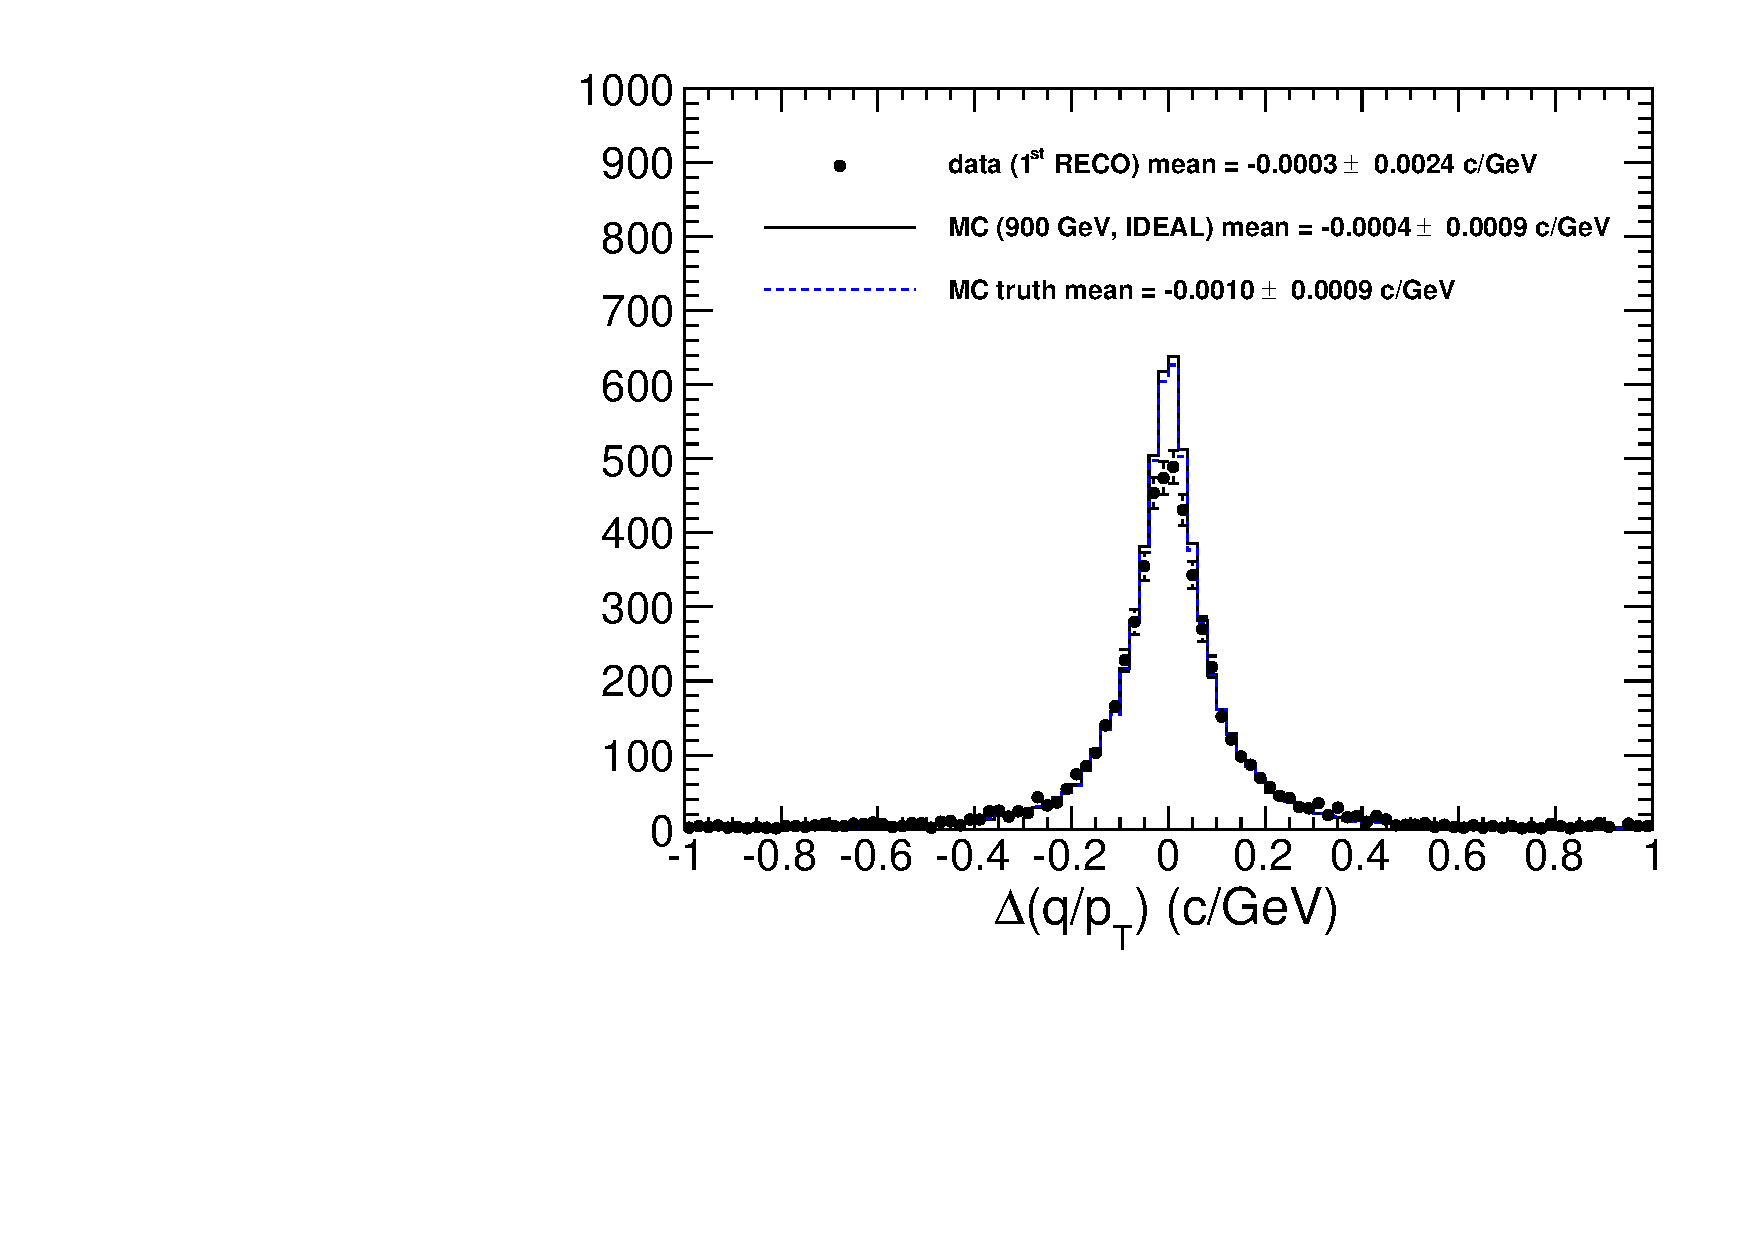
\includegraphics[width=0.5\linewidth]{kaonTracking2_deltaqoverpt.pdf}
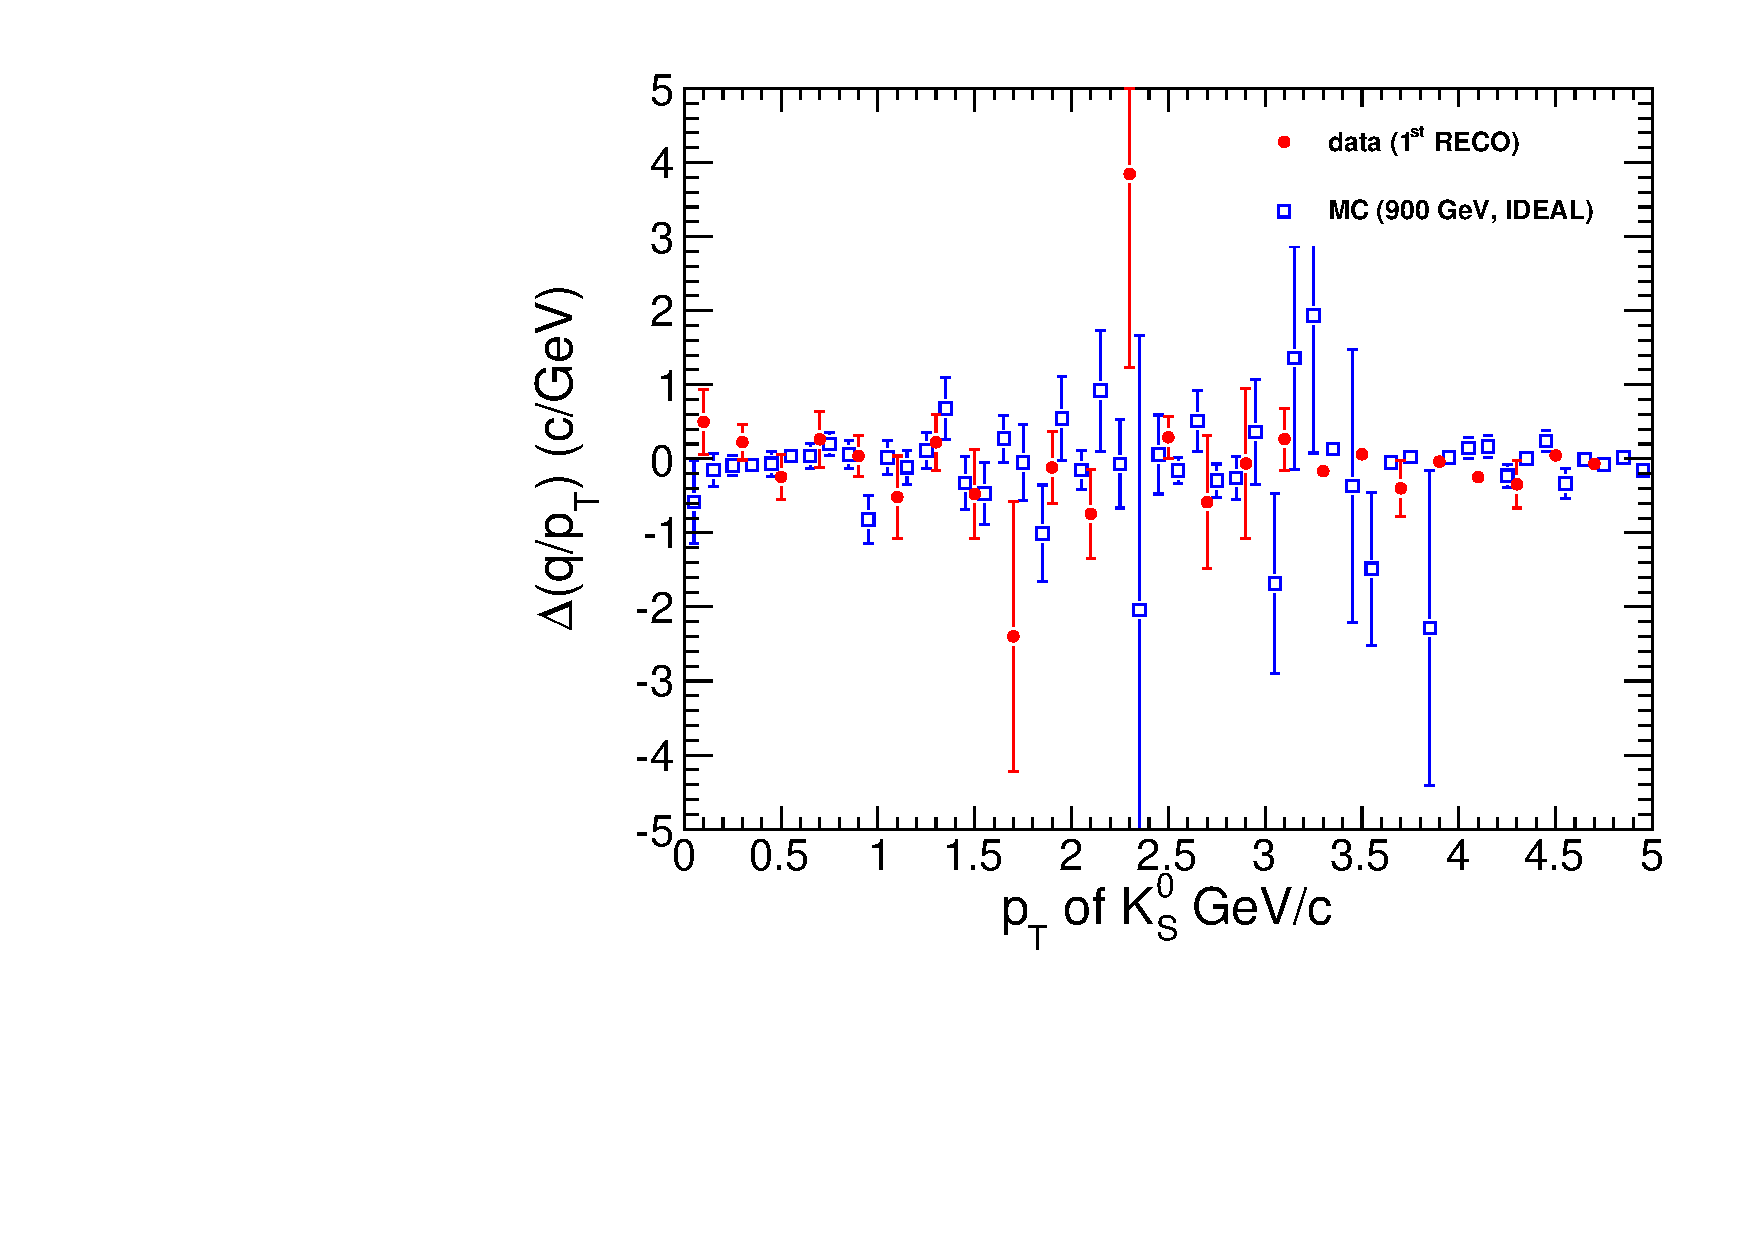
\includegraphics[width=0.5\linewidth]{kaonTracking2_deltaqoverpt_vspt.pdf}

\vfill
\begin{itemize}
\item $\Delta \kappa(\mbox{low}) = -0.000\,3 \pm 0.002\,4$~GeV$^{-1}$
\item 0.24\% uncertainty in bias of 1~GeV tracks
\item Uncertainty in bias of 1~TeV tracks = 240\% (plus a few percent from the $\Delta \kappa(\mbox{high}) - \Delta \kappa(\mbox{low})$ propagation)
\end{itemize}
\end{frame}

\begin{frame}
\frametitle{{\large Flat with respect to everything else}}

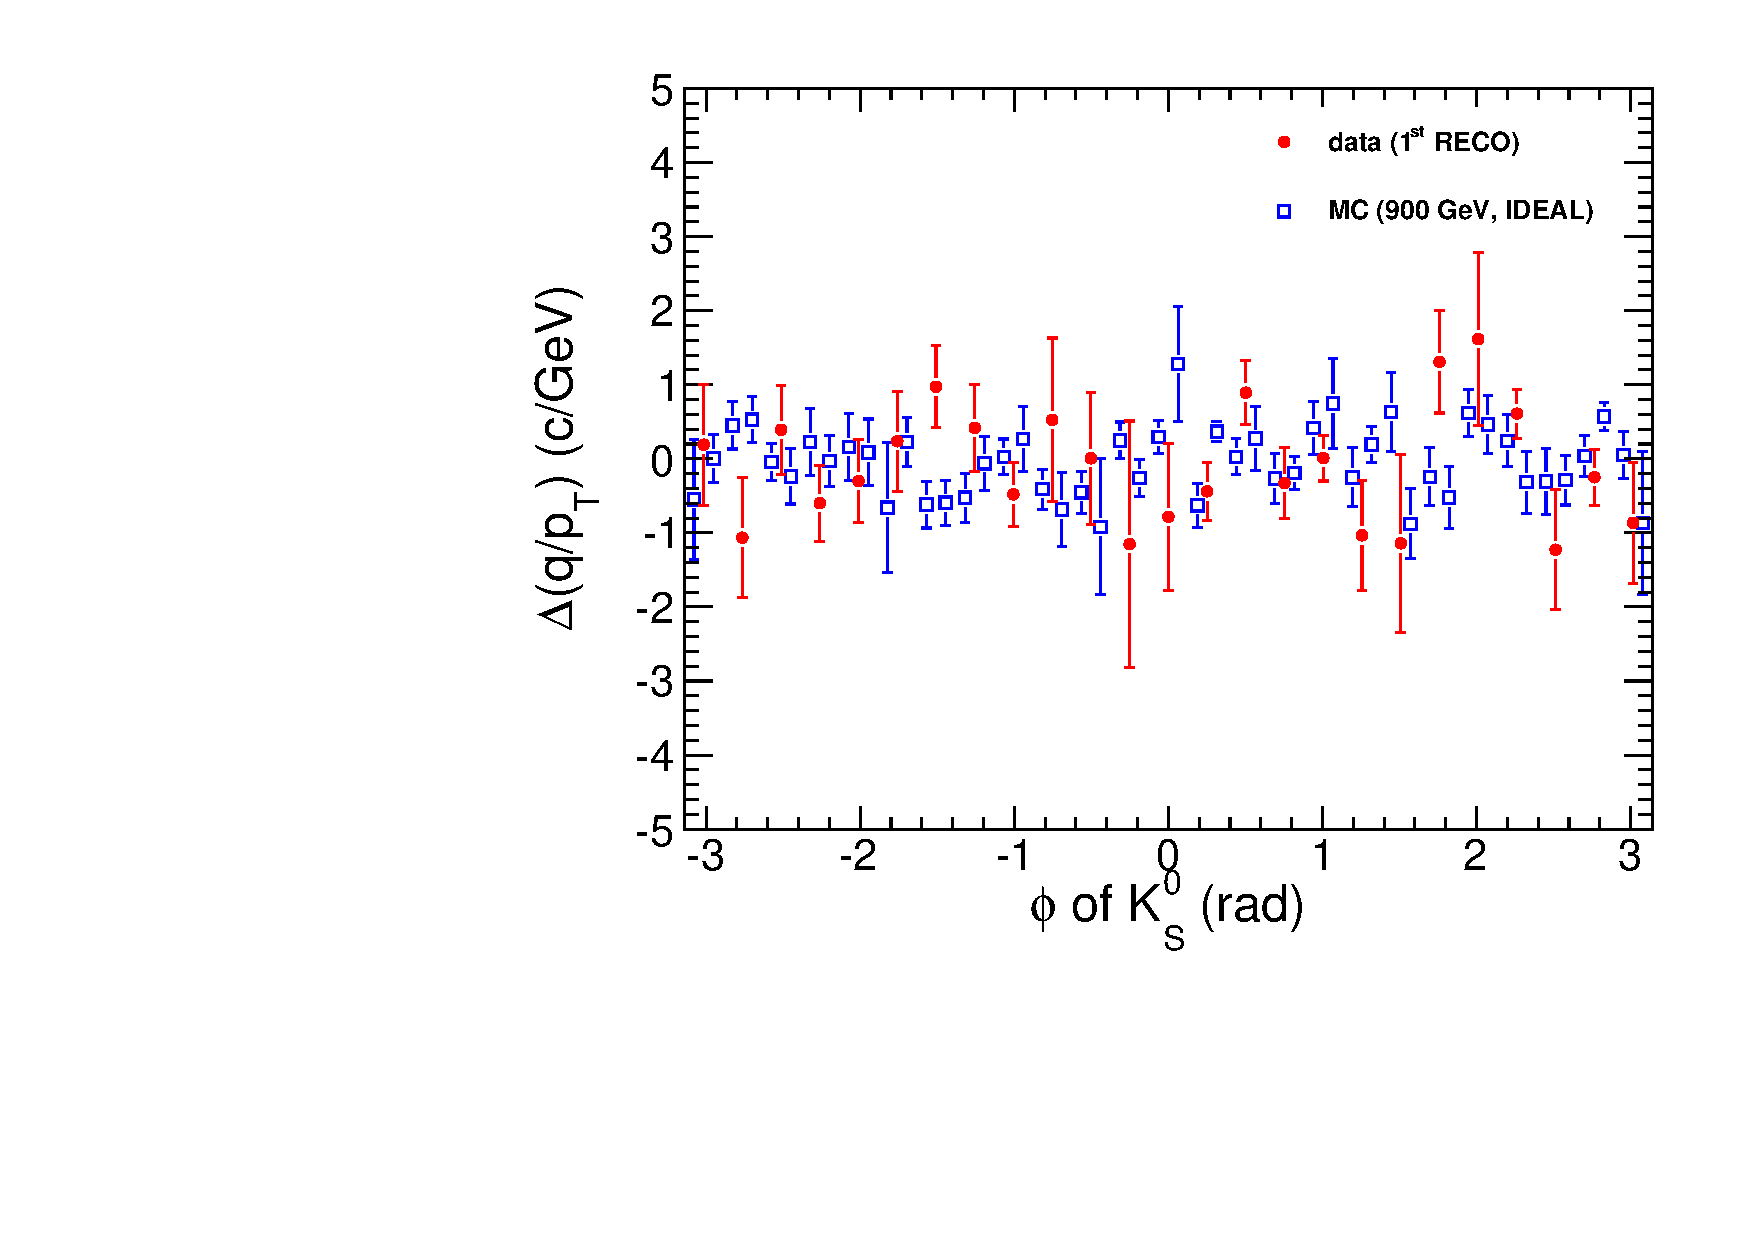
\includegraphics[width=0.32\linewidth]{kaonTracking2_deltaqoverpt_vsphi.pdf}
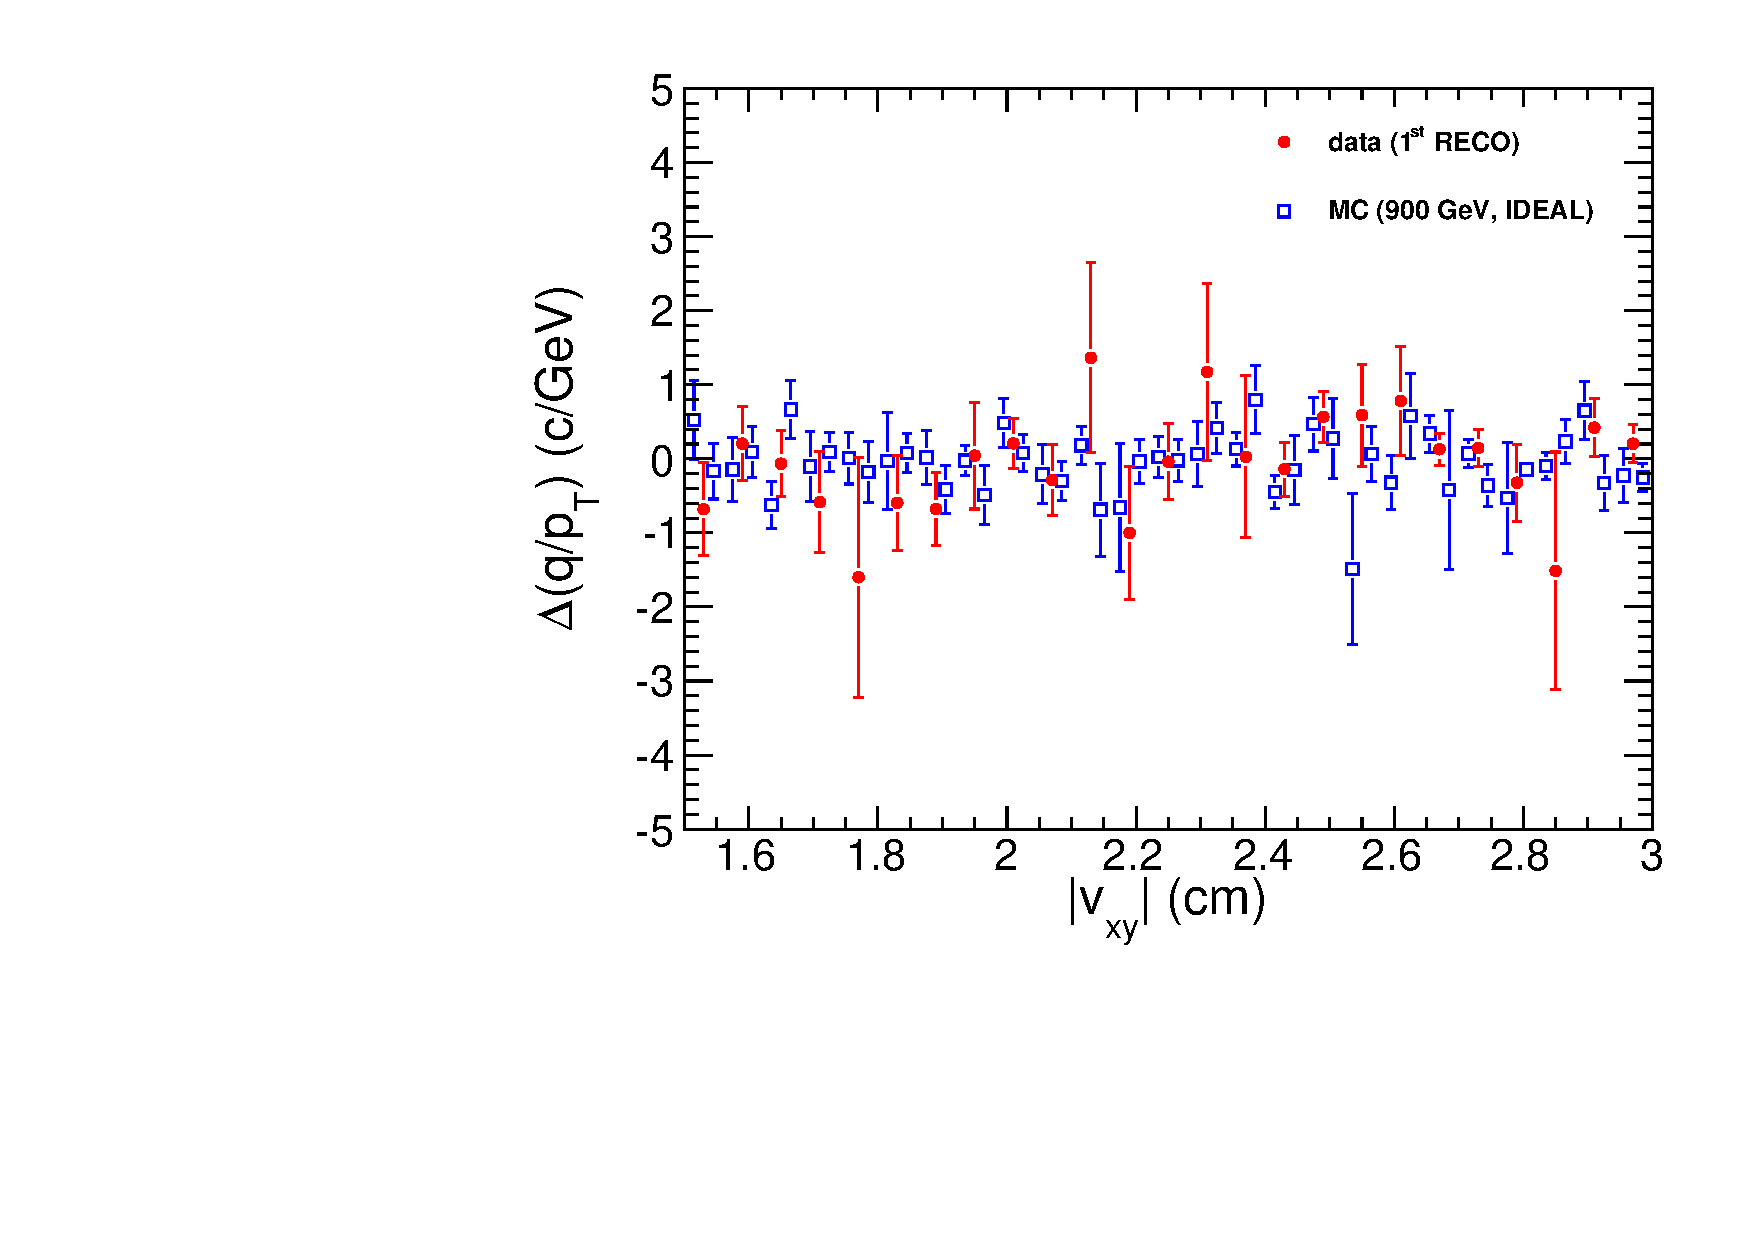
\includegraphics[width=0.32\linewidth]{kaonTracking2_deltaqoverpt_vsvxy.pdf}
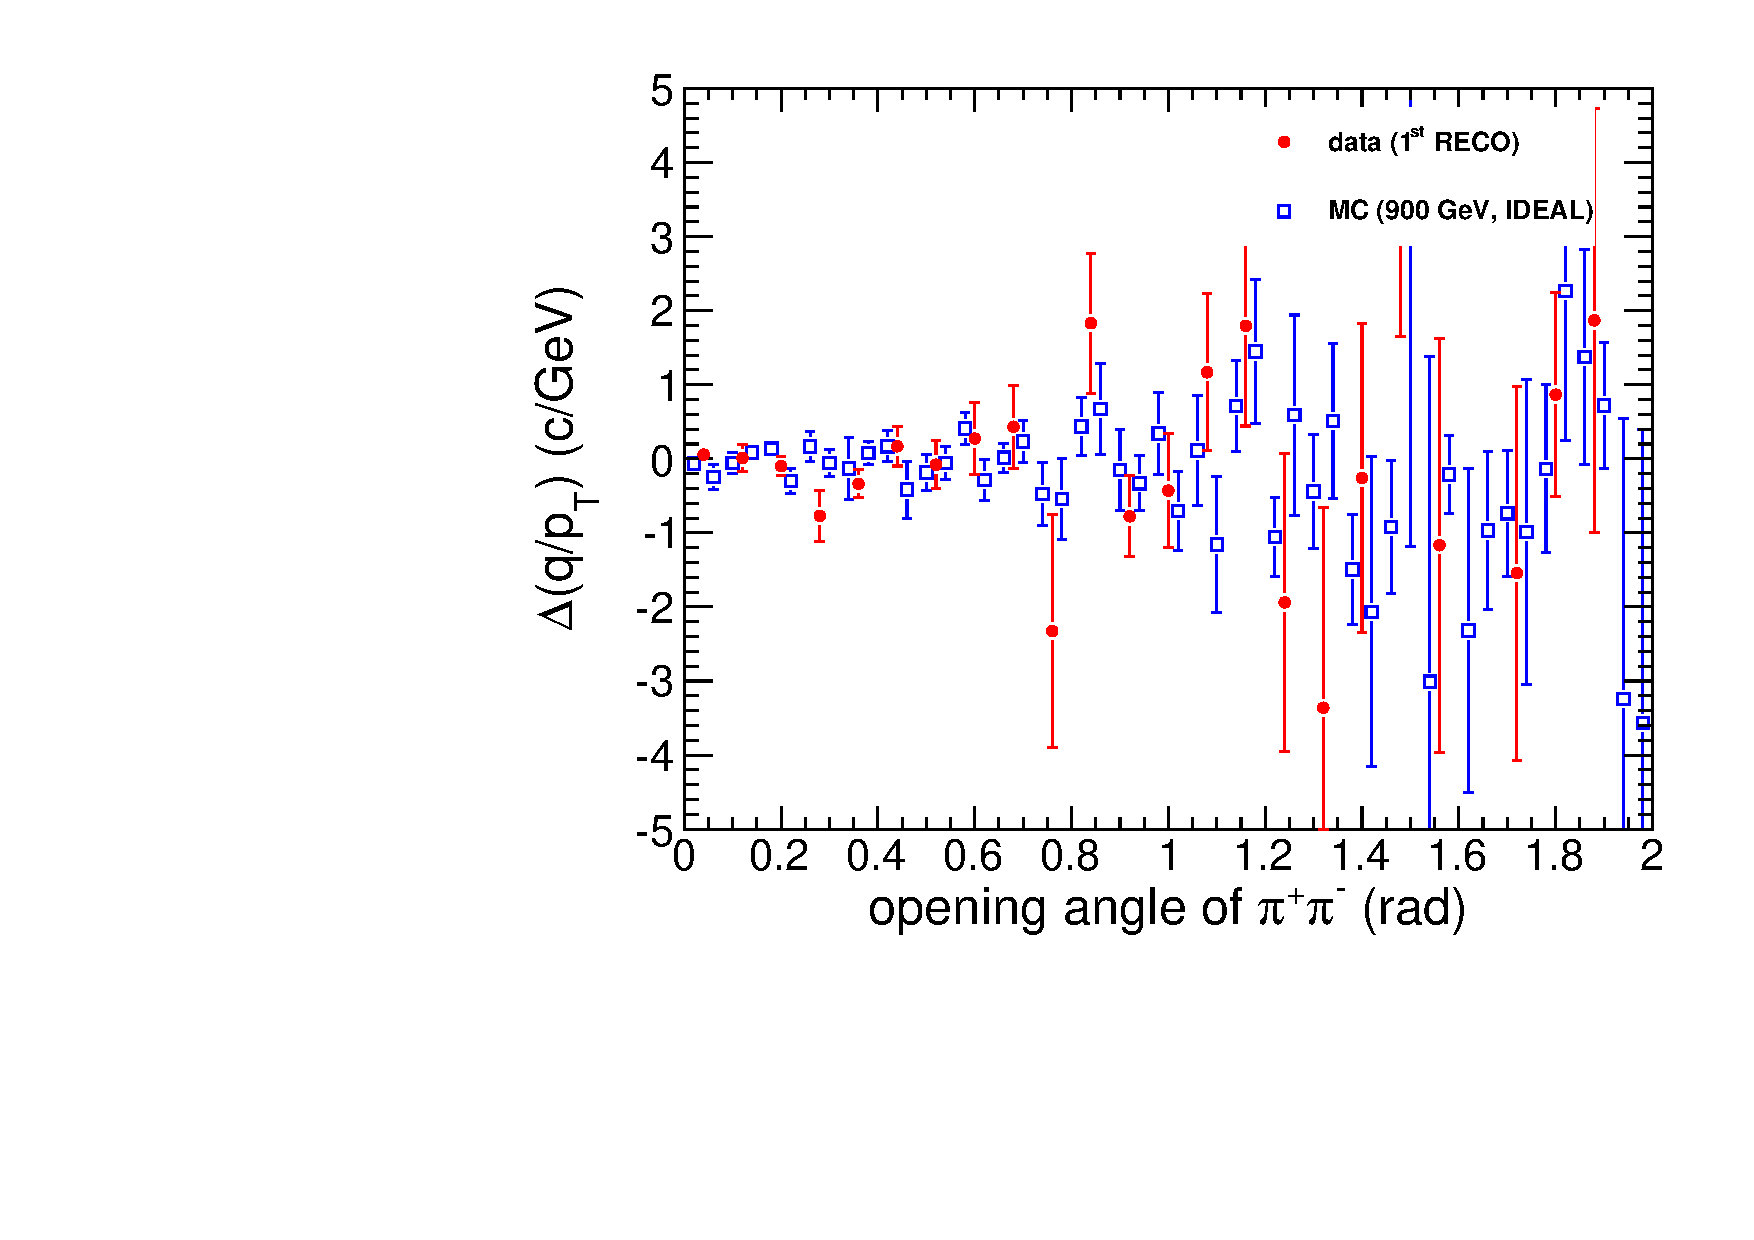
\includegraphics[width=0.32\linewidth]{kaonTracking2_deltaqoverpt_vsopening.pdf}

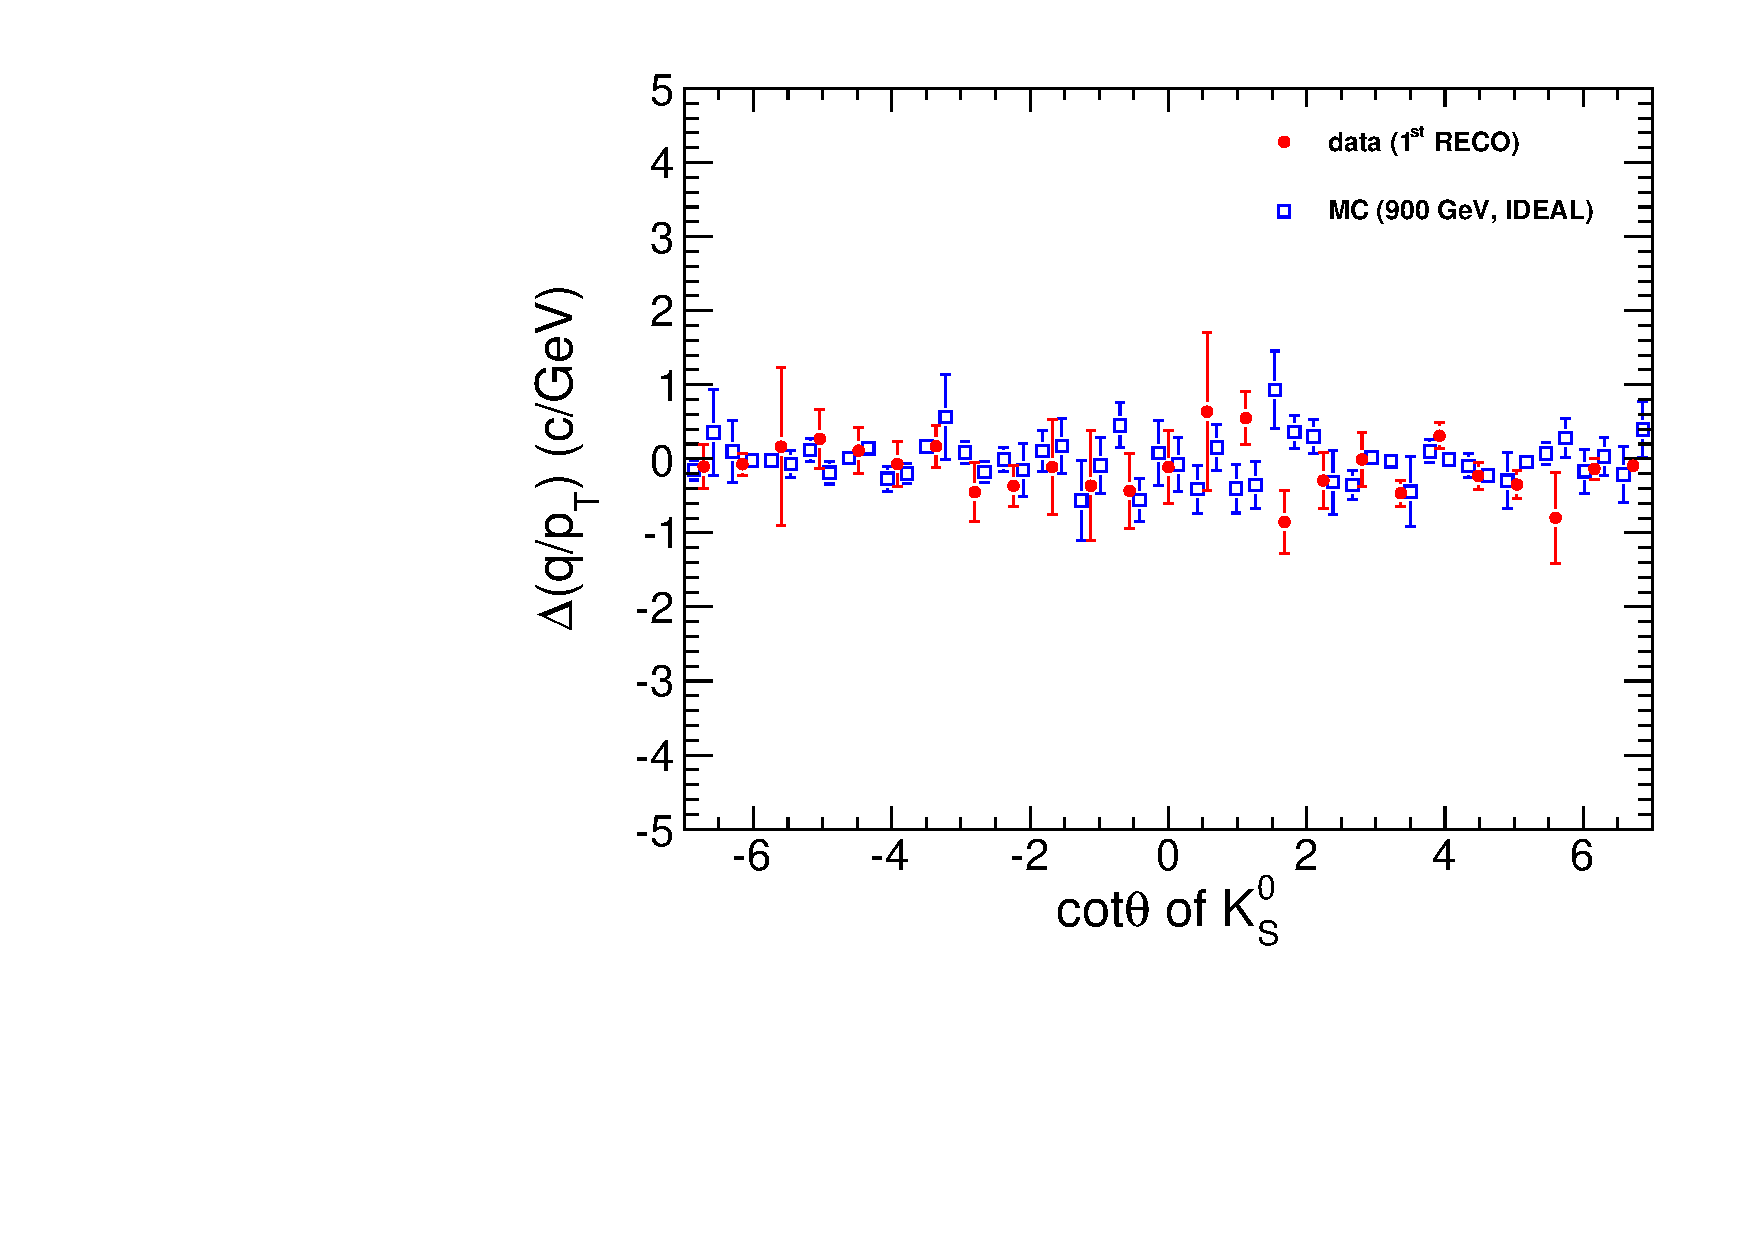
\includegraphics[width=0.32\linewidth]{kaonTracking2_deltaqoverpt_vscottheta.pdf}
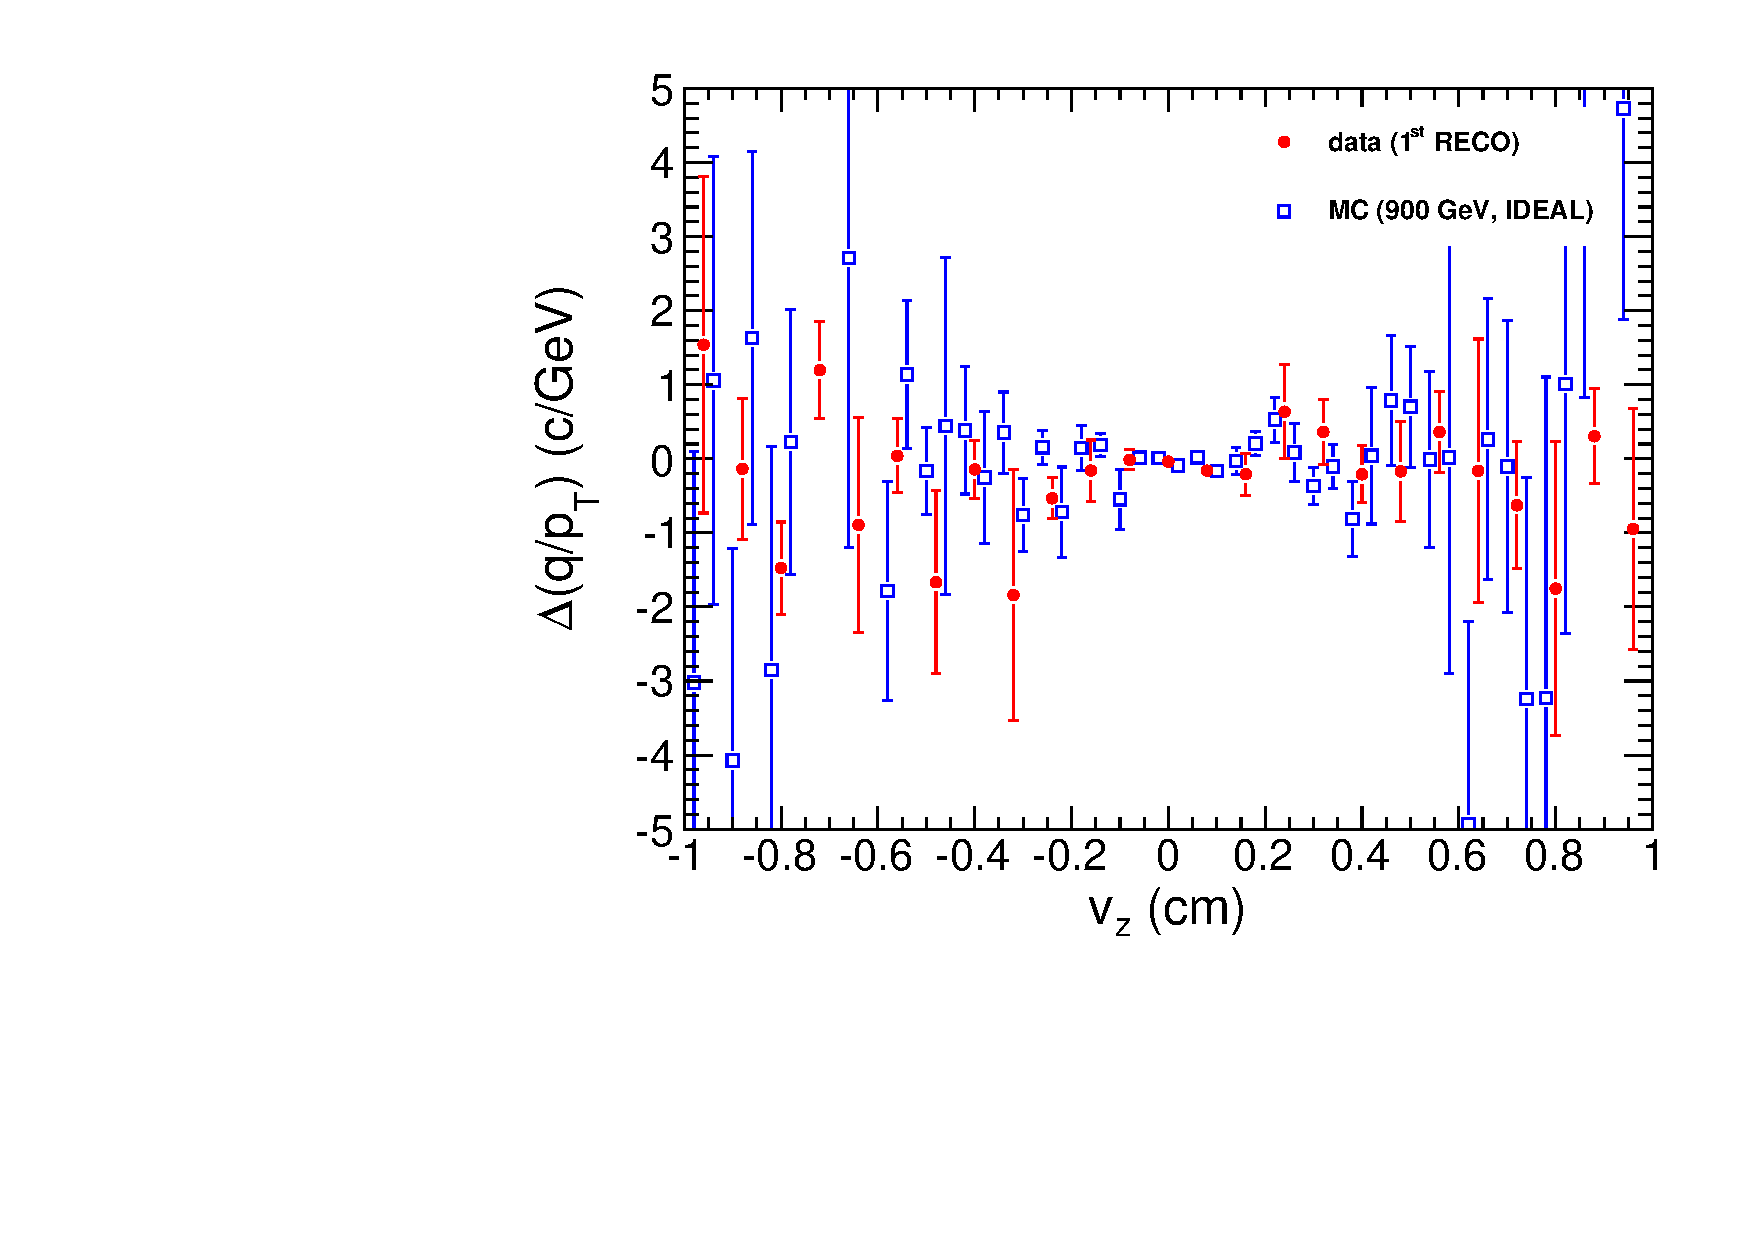
\includegraphics[width=0.32\linewidth]{kaonTracking2_deltaqoverpt_vsvz.pdf}
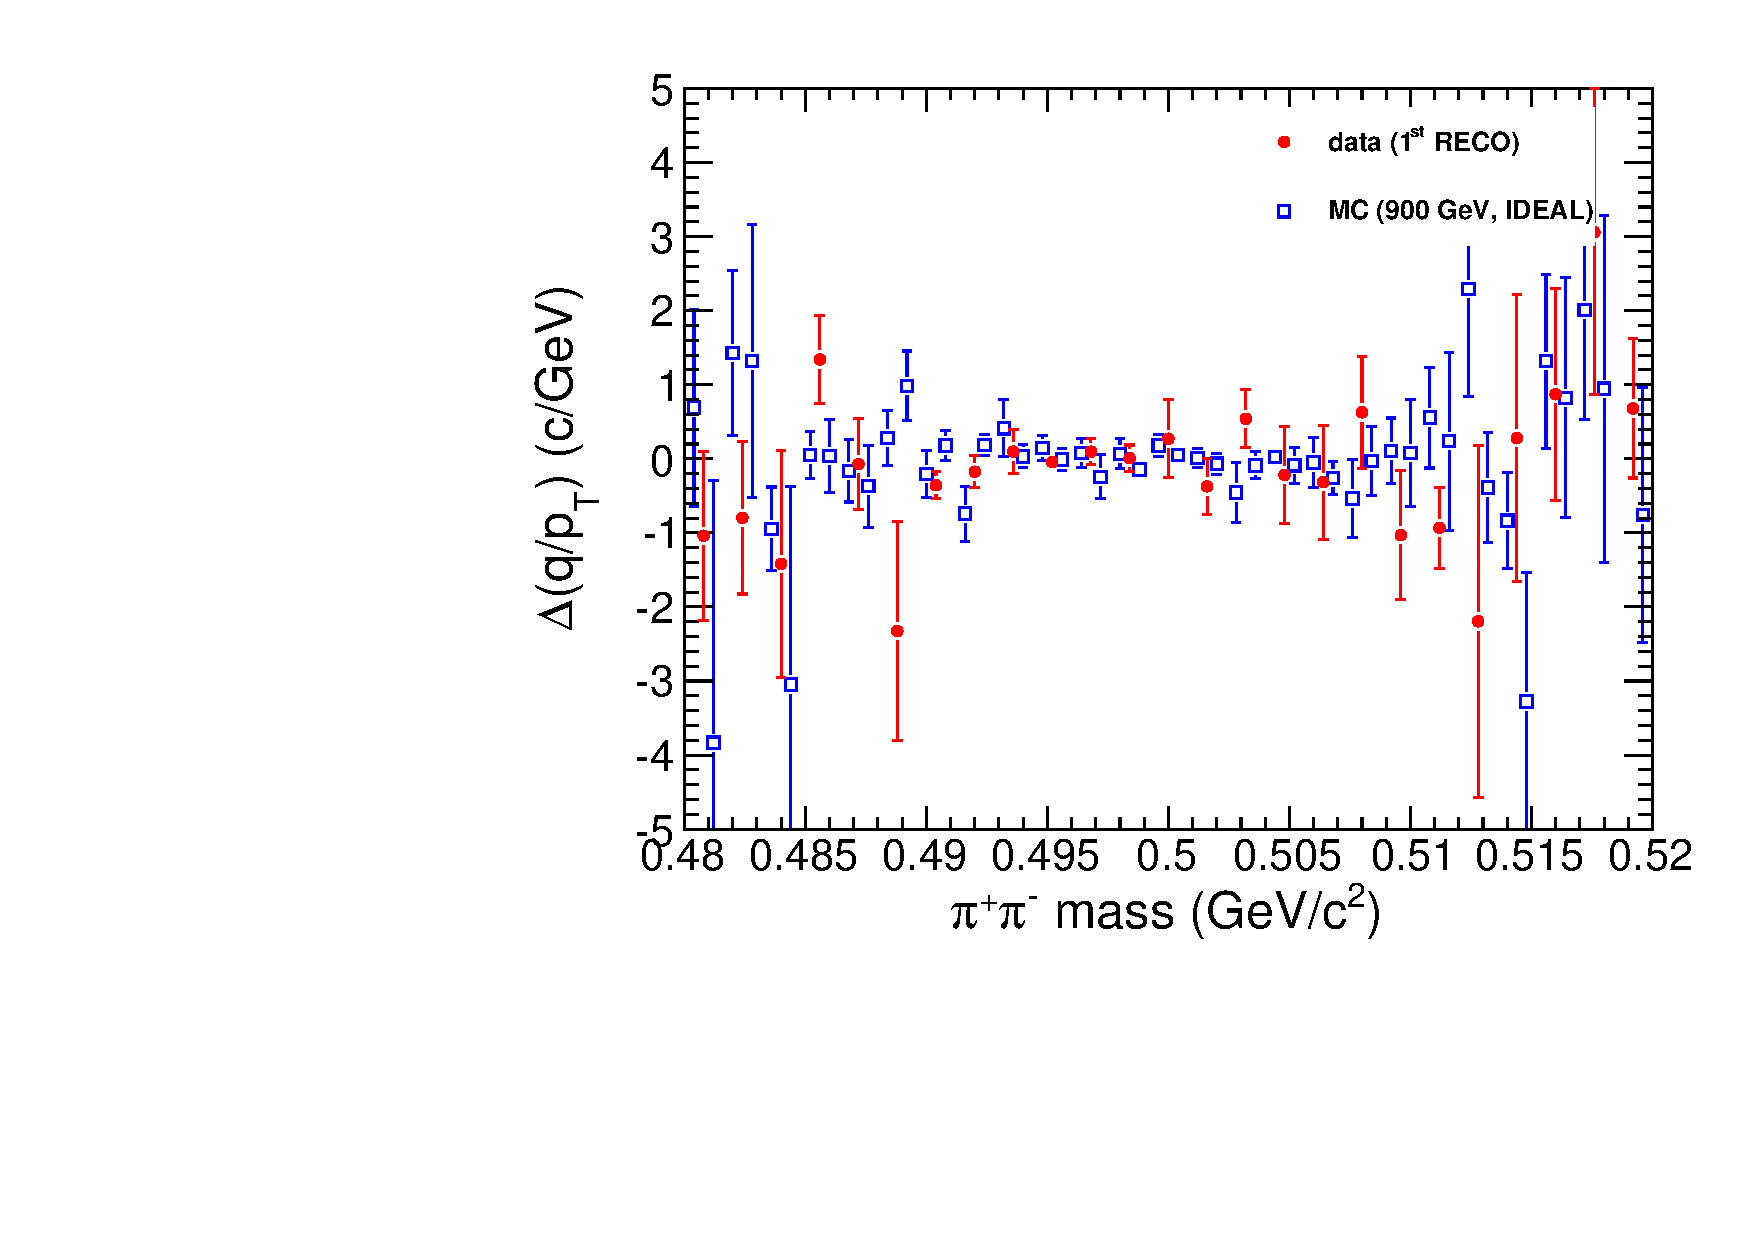
\includegraphics[width=0.32\linewidth]{kaonTracking2_deltaqoverpt_vsmass.pdf}
\end{frame}

\end{document}
